\documentclass[mcp]{article}
%\documentclass[11pt, twocolumn]{article}

\usepackage[colorinlistoftodos]{todonotes}
\usepackage{graphicx}
\graphicspath{ {./images/} }

%\usepackage{fullpage}
\usepackage[margin=1in,headheight=13.6pt]{geometry}
\usepackage{amsfonts,amsthm}
\usepackage{amsmath}
%\numberwithin{figure}{section} % numbering in each subsection
\numberwithin{table}{section}
\usepackage{setspace}
\usepackage{url}
\usepackage{lscape} %% rotating table
\usepackage{rotating}
\usepackage{authblk}
\usepackage{subcaption}
\usepackage{hyperref}
\usepackage{xcolor} %\[table,dvipsnames]
%\usepackage{makecell}
%\usepackage{array}

% remove number of section in the title
\makeatletter
\def\@seccntformat#1{%
  \expandafter\ifx\csname c@#1\endcsname\c@section\else
  \csname the#1\endcsname\quad
  \fi}
\makeatother

\usepackage{caption}

%% to remove zero preceding section number.
\renewcommand\thesection{\arabic{section}}
\renewcommand\thesubsection{\thesection.\arabic{subsection}}

\usepackage{tabulary,multirow,multicol,rotating}
\usepackage[backend=biber, citestyle=numeric, bibstyle=authoryear, sorting=none]{biblatex}
\addbibresource{bibliography.bib}

\makeatletter
\input{numeric.bbx}
\makeatother

\definecolor{Red}{rgb}{0.60,0.00,0.00}
\definecolor{Blue}{rgb}{0.00,0.00,0.75}
\definecolor{LightYellow}{rgb}{1.00,0.97,0.68}
\definecolor{Green}{rgb}{0.30, 0.60, 0.30}
\definecolor{MyLightMagenta}{cmyk}{0.1,0.8,0,0.1} 
\definecolor{cornflowerblue}{rgb}{0.39, 0.58, 0.92}
\definecolor{darkorange}{rgb}{0.8, 0.4, 0}
\definecolor{LightPurple}{rgb}{1, 0.51, 0.98}
\definecolor{DarkPurple}{rgb}{0.54, 0.27, 0.53}
\definecolor{Purple1}{rgb}{0.83, 0.29, 0.95}
\definecolor{Purple2}{rgb}{0.97, 0.12, 0.59}
\definecolor{change}{rgb}{0.39, 0.58, 0.92}

\definecolor{function}{RGB}{0, 112, 192}
\definecolor{group}{rgb}{0.39, 0.58, 0.92}
\definecolor{ratio}{rgb}{1, 0.6, 0.16}
\definecolor{feature}{rgb}{0.83, 0.32, 0.48}
\definecolor{subject}{rgb}{0.6, 0.3, 0.09}
\definecolor{run}{rgb}{0, 0.68, 0.17}

\usepackage{array}
\newcolumntype{C}[1]{>{\centering\let\newline\\\arraybackslash\hspace{0pt}}m{#1}}
\setlength{\tabcolsep}{2pt}

%% for comments
\newcommand{\ignore}[1]{}
\def\todo#1{{\color{red}[#1]}}
\def\change#1{{\color{cornflowerblue}#1}}
\newenvironment{todolong}{\color{red}[TODO:}{]}
\def\ov#1{{\color{red}#1}}
\def\note#1{{\color{OliveGreen}[NOTE: #1]}}
\def\added#1{{\color{blue}[ADDED: #1]}}
\def\devon#1{{\color{green}[4Devon: #1]}}

\def\eqref#1{Eq.~(\ref{eq:#1})}
\def\figshortref#1{{\bf Fig.~\ref{fig:#1}}}
\def\figref#1{{\bf Figure~\ref{fig:#1}}}
\def\secref#1{{\bf Section~\ref{sec:#1}}}
\def\tabref#1{{\bf Table~\ref{tab:#1}}}

\usepackage{xr}
\externaldocument[supp-]{../supplementary/ptm_sm}
%\def\sfigref#1{{\bf Supplementary Fig.~\ref{fig:#1}}}
%\def\snoteref#1{{\bf Supplementary Note~\ref{sec:#1}}}
%\def\snoteshortref#1{{\bf Suppl. Note~\ref{sec:#1}}}
%\def\stabref#1{{\bf Supplementary Table~\ref{tab:#1}}}

%%% should be change =2
\linespread{1}

\usepackage{fancyhdr}
\pagestyle{fancy}
\fancyhead[L]{MSstatsPTM: Statistical relative quantification of PTMs}

%\date{\vspace{-5ex}} % to remove date in the title

\renewcommand{\deg}{\ensuremath{^{\circ}}\xspace}
\newcommand{\dd}[1]{\mathrm{d}#1}

%%%%%%%%%%%%%%%%%%%%%%%%%%%%%%%%%%%%%%%%%%%%%%%%%%%%%%%%%%%%%%%%%%%%%%%
%%%%%%%%%%%%%%%%%%%%%%%%%%%%%%%%%%%%%%%%%%%%%%%%%%%%%%%%%%%%%%%%%%%%%%%
%%%%%%%%%%%%%%%%%%%%%%%%%%%%%%%%%%%%%%%%%%%%%%%%%%%%%%%%%%%%%%%%%%%%%%%

\title{MSstatsPTM: Statistical relative quantification of post-translational modifications in bottom-up mass spectrometry-based proteomics}

\author[1]{Devon~Kohler}
\author[2]{Tsung-Heng~Tsai}
\author[4]{Erik~Verschueren}
\author[1]{Ting~Huang}
\author[3]{Trent~Hinkle}
\author[3]{Lilian~Phu}
\author[3]{Meena~Choi*}
\author[1]{Olga~Vitek*}
\affil[1]{Khoury College of Computer Science, Northeastern University, Boston, MA, USA}
\affil[2]{Kent State University, Kent, OH, USA}
\affil[3]{MPL, Genentech, South San Francisco, CA, USA}
\affil[4]{ULUA BV, Arendstraat 29, 2018 Antwerp, Belgium}
\affil[*]{Corresponding Authors}
%\affil[]{MSstatsPTM: Statistical relative quantification of PTMs}

\date{}

\begin{document}

\maketitle


%%%%%%%%%%%%%%%%%%%%%%%%%%%%%%%%%%%%%%%%%%%%%%%%%%%%%%%%%%%%%%%%%%%%%%%
%%%%%%%%%%%%%%%%%%%%%%%%%%%%%%%%%%%%%%%%%%%%%%%%%%%%%%%%%%%%%%%%%%%%%%%
\begin{abstract}

Liquid chromatography coupled with bottom up mass spectrometry (LC-MS/MS)-based proteomics is increasingly used to detect changes in post-translational modifications (PTMs) in samples conditions. Analysis of data from such experiments faces numerous statistical challenges. These include the low abundance of modified proteoforms, the small number of observed peptides that span modification sites, and confounding between changes in the abundance of PTM and the overall changes in the protein abundance. Therefore, statistical approaches for detecting differential PTM abundance must integrate all the available information pertaining to a PTM site, and consider all the relevant sources of confounding and variation. In this manuscript we propose such a statistical framework, which is versatile, accurate, and leads to reproducible results. The framework requires an experimental design, which quantifies, for each sample, both peptides with post-translational modifications and peptides from the same proteins with no modification sites. The proposed framework supports both label-free and tandem mass tag (TMT)-based LC-MS/MS acquisitions. The statistical methodology separately summarizes the abundances of peptides with and without the modification sites, by fitting separate linear mixed effects models appropriate for the experimental design. Next, model-based inferences regarding the PTM and the protein-level abundances are combined to account for the confounding between these two sources. Evaluations on computer simulations, a spike-in experiment with known ground truth, and three biological experiments with different organisms, modification types and data acquisition types demonstrate the improved fold change estimation and detection of differential PTM abundance, as compared to currently used approaches. The proposed framework is implemented in the free and open-source R/Bioconductor package $MSstatsPTM$. 

\end{abstract}

%%%%%%%%%%%%%%%%%%%%%%%%%%%%%%%%%%%%%%%%%%%%%%%%%%%%%%%%%%%%%%%%%%%%%%%
%%%%%%%%%%%%%%%%%%%%%%%%%%%%%%%%%%%%%%%%%%%%%%%%%%%%%%%%%%%%%%%%%%%%%%%
\clearpage
\section{Introduction}

Signaling mechanisms allow cells to mount a fast and dynamic response to a multitude of biomolecular events. Signaling is facilitated by the modification of proteins at specific residues, acting as molecular on/off switches~\cite{Deribe,Cohen,Bludau2022}. Characterizing relative abundance of a modification site's occupancy repertoire across experimental conditions provides important insights~\cite{Mann}. For example, meaningful patterns of changes in post-translational modifications (PTMs) abundance can serve as biomarkers of a disease~\cite{Petushkova_2017}. Alternatively, distinguishing the quantitative changes in a PTM from the overall changes of the protein abundance helps gain insight into biological and physiological processes operating on a very short timescale~\cite{Wu:2011, Chandramouli:2009, Kim2016}. This helps to distinguish between relative site occupancy changes at steady-state protein levels, typical for short time-scale signaling events, and observed relative changes of PTMs as a result of underlying gene expression or protein abundance levels.

Bottom-up liquid chromatography coupled with tandem mass spectrometry (LC-MS/MS) is a tool of choice for unbiased and large-scale identification and quantification of proteins and their PTMs~\cite{Kall:2011ub,Roepstorff}. However, LC-MS-based interrogation of the modified proteome is challenging, for a number of reasons. First, the relatively lower abundance of modified proteoforms dictates that a global interrogation can only be achieved through large-scale enrichment protocols with modification-specific antibodies or beads \cite{Huang:2014}. Variability in the enrichment efficiency inevitably affects the reproducibility of the number of spectral features (e.g., peptide precursor ions or their fragments) and their intensities. Second, contrary to the often large number of identified peptides that can be used to quantify protein abundance, there are relatively few representative peptides that span a modification site, and there may be multiple modified sites on a single peptide~\cite{Mann}. Third, unless early signaling events are interrogated, the interpretation of the relative changes in modification occupancy are inherently confounded with changes in the overall protein abundance, complicating the interpretation of the results \cite{Wu:2011, Olsen:2013}. Finally, technological aspects of bottom-up MS experiments, such as presence of labeling by tandem mass tag (TMT), introduce additional sources of uncertainty and variation.

The technological difficulties in PTM identification and quantification increase the uncertainty and the variation in the data, and challenge the downstream statistical analyses. Frequently data from these experiments are analyzed using statistical methods that were not originally designed for this task. Researchers use methods such as $t$-test\cite{Kalpic:2011}, Analysis of Variance (ANOVA)\cite{girden:1992}, or Limma\cite{Ritchie_15a}, by taking as input the intensity ratios of modified and unmodified peptide features, and comparing the mean abundance of different PTM sites. Such approaches do not fully account for all the sources of uncertainty. As the result, these approaches are either not directly applicable to experiments with non-trivial designs (such as experiments with multiple conditions, paired and time course designs, and experiments with labeling), or require the analysts to exercise non-trivial statistical expertise.

This manuscript proposes a versatile statistical analysis framework that accurately detects relative changes in post-translational modifications. The framework requires an experimental design, which quantifies, for each sample, both the peptides with post-translational modifications, and peptides from the same proteins with no modification sites. The framework supports data-dependent acquisitions (DDA) that are label-free or tandem mass tag (TMT)-based. The statistical methodology separately summarizes the abundances of peptides with and without the modification sites, and fits separate linear mixed effects models that reflect the biological and technological aspects of the experimental design. Next, model-based inferences regarding the PTM and the unmodified protein-level abundances are combined to account for the confounding between these two sources.

We evaluated the proposed framework on two datasets from computer simulations, one benchmark controlled mixture, and three biological investigations. The datasets illustrate a diverse set of organisms, modification types, acquisition methods and experimental designs, showing the applicability of the framework to a variety of situations. By appropriately leveraging the information from the unmodified proteins, the proposed approach improved the accuracy of the estimates of PTM fold changes, and produced a better calibrated false positive rate of detecting differentially abundant PTMs as compared to existing methods. In particular, accounting for the confounding from unmodified protein abundance allowed us to characterize the true effect of the modification, avoiding the need for more manual and time intensive follow-up investigation.

The proposed approach is implemented as a freely available open source R package $MSstatsPTM$, as part of the $MSstats$ family of packages \cite{Choi:2014,Huang:2020}, and is available on Bioconductor.

\section{Experimental procedures}

\subsection*{Data overview and availability}

Table \ref{tab:dataDescription} summarizes the experiments. Two computer simulations had known ground truth, and varied in experimental realism. The first simulation produced a perfectly clean dataset, with many replicates and no missing values. The second simulation introduced real-world characteristics, such as limited modified features and missing values. Details of computer simulations are available in Supplementary Section \ref{supp-sec:sim} and on GitHub (\url{https://github.com/devonjkohler/MSstatsPTM_simulations}).

One spike-in experiment also had known changes in modified spike-in peptides, but had real-world experimental characteristics. Finally, three biological experiments demonstrated the applicability of the proposed approach across different biological organisms, modifications, experimental designs and acquisition strategies. The experimental data, R scripts with $MSstatsPTM$ analysis, and results of the statistical analysis are available in MassIVE.quant (\url{https://massive.ucsd.edu/ProteoSAFe/static/massive-quant.jsp}) \cite{Choi:2020}. 

\subsection*{Dataset 1: Computer simulation 1 - Label-free}
\label{sec:comp_sim_procedure1}

{\bf Simulation design:} The simulation represented an idealistic case. 24 synthetic label-free datasets were generated with different experimental designs and different biological variation. In each dataset, 1,000 proteins had 10 unmodified features per protein. Each of the 1,000 proteins had one PTM. Each PTM was represented by 10 modified features. The PTMs of 500 proteins had a differential fold change between conditions, while the other 500 proteins were generated with no changes in abundance between conditions. Furthermore, the fold changes of half of the 500 differential PTMs were fully masked by changes in the unmodified protein. Finally, the fold change of half the 500 non-differential PTMs was entirely due to changes in the unmodified protein. All the differential PTMs were generated with an expected log base 2 fold change of 0.75 between conditions. 

Each simulation was generated with random biological variation. The observed peptide abundances were simulated by adding random noise $\mathcal{N}(0,\sigma^2)$ to the deterministic abundances described above. Two values $\sigma^2 = \{.2, .3\}$ were motivated by the experimental datasets in this manuscript.

\medskip \noindent {\bf Evaluation:} We evaluated the ability of the statistical methods to correctly detect differentially abundant PTMs. We gauged the methods ability to avoid false positives (i.e. specificity), accurately estimate the fold change between conditions, and analyzed the sensitivity of detecting differentially abundant PTMs. The evaluation was performed both in the presence of confounding with changes in the unmodified protein and after applying adjustment to correct for the confounding.

\subsection*{Dataset 2: Computer simulation 2 - Label-free missing values and low features}
\label{sec:comp_sim_procedure2}

{\bf Simulation design:} The data were simulated as above, while providing a more realistic representation of the experiments. The feature counts and the proportion of missing values were as observed on average over all the the experimental datasets in this manuscript. Specifically, PTMs were simulated with 2 modified peptide features, and unmodified proteins were simulated with 10 features. Additionally, 20\% of observations for both modified and unmodified peptides were missing completely at random.

\medskip \noindent {\bf Evaluation:} The methods were evaluated as above. We evaluated their ability to correctly detect PTM's specificity, fold change estimation, and sensitivity. These statistics were analyzed both in the presence of, and without, confounding with the overall changes in protein abundance.
 
\subsection*{Dataset 3: Spike-in benchmark - Ubiquitination - Label-free}
\label{sec:exp_proc_dataset3}

\medskip \noindent {\bf Experimental design:}~\figref{benchmark-design}(a) overviews the experimental design. Four mixtures (i.e., conditions) were created with varying amounts of human lysate, background {\it E. Coli} lysate, and human spike-in ub-peptide mixture. Unmodified peptides from human lysate were viewed as the global proteome. Background {\it E. coli} lysate were used to equalize total protein levels.   50 heavy-labeled KGG motif peptides from 20 human proteins were spiked into the mixed background of the lysates. Quantitative changes in protein and site abundance of these 20 human proteins were the target of the benchmark. In particular, we distinguished the unadjusted changes (i.e. changes in the abundances of the modified peptides) and the protein-level adjusted changes of (i.e., changes in the abundances of the modified peptides relative to the changes in the abundances of the human lysate). The true log-fold changes between the relevant components of the relevant mixtures are summarized in~\figref{benchmark-design}(b).  Two replicate mixtures were created per condition. 

\medskip \noindent {\bf Data acquisition:} Each mixture was analyzed with KGG enrichment, and without KGG enrichment (i.e., in a global profiling run), with label-free LC-MS/MS. There was a 90.2\% overlap of protein identifications between the identified background modified peptides and proteins quantified in the global profiling run.

\medskip \noindent {\bf Evaluation:} We expect the relative abundances of the spike-in peptides to change as in~\figref{benchmark-design}(b). The changes in peptide abundances in all the comparisons except Mix 4 vs Mix 1 were distinct from changes in the global proteome abundances and distinct from zero, and were viewed as positive controls. In the comparison of Mix4 vs Mix 1 both the modified peptides and the global proteome background changed two-fold, and as the result the peptides in this comparison were viewed as a negative control. The background {\it E. Coli} lysate peptides were not expected to change in abundance in comparison, after accounting for adjustment, and were viewed as additional negative controls. We evaluated the statistical methods ability to avoid false positives, as well as their sensitivity in detecting the differentially abundant spike-in peptides and accurately estimate their expected fold change.


\subsection*{Dataset 4: Human - Ubiquitination - 1mix-TMT}
\label{sec:exp_proc_dataset4}

\medskip \noindent {\bf Experimental Design:}  Luchetti et al.~\cite{LUCHETTI2021} profiled human epithelial cells engineered to express IpaH7.8 under a dox inducible promoter. Uninfected cells were measured at 0 and 6 hours, while cells infected with {\it Shigella Flexneri} ({\it S. Flexneri}) bacteria were measured at 1, 2, 4, and 6 hour increments, resulting in six total conditions. 11 samples were allocated to 1 TMT mixture in an unbalanced repeated measure design. All conditions had two biological replicates except for the Dox1hr condition, which was allocated one replicate.

\medskip \noindent {\bf Data acquisition:} The ubiquitinated peptides, and the total proteome (i.e., global profiling) were each conducted in a single LC-MS/MS run. There was a 95\% overlap between the identified modified peptides and proteins that were quantified in the global profiling run.

\medskip \noindent {\bf Evaluation:} We evaluated the ability of the statistical methods to detect changes in the abundance of modified peptides both before and after adjusting for changes in global protein abundance. The six condition were labeled Dox1hr, Dox2hr, Dox4hr, Dox6hr, NoDox0hr, and NoDox6hr. All conditions were compared with each other, resulting in 15 pairwise comparisons. Since the dataset was a biological investigation, the true positive modifications were unknown. Shigella ubiquitin ligase IpaH7.8 was shown to function as an inhibitor of the protein Gasdermin D (GSDMD). GSDMD was actively degraded when IpaH7.8 expression was induced by dox treatment in human cells. We expect IpaH7.8 to function as an inhibitor of GSDMD in the global profiling run.

\subsection*{Dataset 5: Mouse - Phosphorylation - 2mix-TMT}
\label{sec:exp_proc_dataset5}


\medskip \noindent {\bf Experimental Design:} Maculins et al. \cite{Maculins} studied primary murine macrophages infected with {\it S. Flexneri}. The experiment quantified the abundance of total protein and of phosphorylation in wild type (WT), and in ATG16L1-deficient (cKO) samples, uninfected and infected with {\it S. Flexneri}. The abundance of total protein and post-translation modifications were quantified at three time points, uninfected, early infection (45-60 minutes), and late infection (3-3.5 hours). 22 biological samples were allocated to 2 TMT mixtures in an unbalanced repeated measure design, with 11 samples allocated to each mixture. 16 replicates were spread equally between the early and late WT and cKO conditions, resulting in four replicates per condition. Both the uninfected WT and cKO contained 3 replicates, with mixture one allocating one replicate to uninfected WT and two replicates to uninfected cKO. Conversely, mixture two contained one replicate of uninfected cKO and two uninfected WT.

\medskip \noindent {\bf Data acquisition:} This experiment included a total proteome (i.e., a global profiling run) and a phosphopeptide enrichment run. There was a 90\% overlap between the identified modified peptides and proteins that were quantified in the global profiling run.

\medskip \noindent {\bf Evaluation:} We evaluated the ability of the statistical methods to detect changes in the abundance of modified peptides both before and after adjusting for changes in global protein abundance. The six condition were labeled KO\_Uninfect, KO\_Early, KO\_Late, WT\_Uninfect, WT\_Early, and WT\_Late. 9 total comparisons were made, namely KO\_Early-WT\_Early, KO\_Late-WT\_Late, KO\_Uninfected-WT\_Uninfected, KO\_Early-KO\_Uninfected, KO\_Late-KO\_Uninfected, WT\_Early-WT\_Uninfected, WT\_Late-WT\_Uninfected, Infected-Uninfected, and KO-WT. Since the dataset was a biological investigation, the true positive modifications were unknown.


\subsection*{Dataset 6: Human - Ubiquitination - Label-free no global profiling run}
\label{sec:exp_proc_dataset6}

\medskip \noindent {\bf Experimental Design:} Cunningham et al. \cite{Cunningham2015} investigated the relationship between USP30 and protein kinase PINK1, and their association with Parkinson’s Disease. The experiment profiled ubiquitination sites, and analyzed changes in the modified site abundance. The experiment had four conditions, CCCP, USP30 over expression (USP30 OE), Combo, and Control. Cell lines were used to create two biological replicates per condition. The abundance of modified peptides was quantified with label-free LC-MS/MS.

\medskip \noindent {\bf Data acquisition:} This experiment did not include a separate global profiling run to measure unmodified peptides. In addition to low feature counts for unmodified peptides,  this lead to substantially fewer matches between modified and unmodified peptides. There was a 41.9\% overlap between the identified background modified peptides and proteins that were quantified in the global profiling run.

\medskip \noindent {\bf Evaluation:} We evaluated the ability of the statistical methods to detect  changes in the abundance of modified peptides both before and after adjusting for changes in global protein abundance. All the conditions were compared with each other in a full pairwise comparison, resulting in 6 comparisons. Since the dataset is a biological investigation, the true positive modifications were unknown.

%%%%%%%%%%%%%%%%%%%%%%%%%%%%%%%%%%%%%%%%%%%%%%%%%%%%%%%%%%%%%%%%%%%%%%%
\section*{Background}

\subsection*{Goals of PTM characterization, input to statistical analyses, and notation}

Consider a label-free LC-MS/MS experiment in the special case of a balanced design with $I$ conditions and $J$ biological replicates per condition. For simplicity, we assume that the experiment has no technical replicates, such that each biological replicate is represented by a single LC-MS/MS run.  
\figref{data-structure} schematically illustrates this data structure for one protein and one PTM site, $I=2$ and $J=2$.
For one protein, the PTM site is represented by $K$ spectral features (i.e., peptide ions, distinguished by their cleavage residues and charge states). 
The number of modified and unmodified features typically varies across proteins. Some log-intensities can be outliers, and some spectral features can be missing. 
The log$_2$-intensity of Feature $k$, in Replicate $j$ of Condition $i$ is denoted by $y_{ijk}^{\ast}$. Conversely, the unmodified protein is represented by $L$ spectral features, and the log-intensity of Feature $l$ from the unmodified protein in the same run is denoted by $y_{ijl}$. The features can be quantified as part of a same mass spectrometry run, or in a separate enrichment and global proteome profiling run.

The population quantity of interest is the difference between the log$_2$ abundances of a PTM site in Condition $i$ and Condition $i^{\prime}$, denoted by $\mu_i^{\ast}$ and $\mu_{i^{\prime}}^{\ast}$ respectively. We are interested in testing the null hypothesis
\begin{eqnarray}
H_{0}: \Delta_{PTM} = \mu_{i}^{\ast} - \mu_{i^{\prime}}^{\ast} = 0 \ \text{vs} \ 
H_{a}: \Delta_{PTM} = \mu_{i}^{\ast} - \mu_{i^{\prime}}^{\ast} \neq 0
\label{eq:conv_null_hyp}
\end{eqnarray}
Unfortunately, this population quantity is inherently confounded with the overall changes in protein abundance. To account for this, it is advantageous to consider a different null hypothesis:
\begin{eqnarray}
H_{0}: \Delta_{adj} = ( \mu_{i}^{\ast} - \mu_{i}) - ( \mu_{i^{\prime}}^{\ast} - \mu_{i^{\prime}} ) = 0 \ \text{vs} \ 
H_{a}: \Delta_{adj} = ( \mu_{i}^{\ast} - \mu_{i}) - ( \mu_{i^{\prime}}^{\ast} - \mu_{i^{\prime}} ) \neq 0
\label{eq:null_hyp}
\end{eqnarray}
where $\mu_i$ and $\mu_{i^{\prime}}$ reflect the overall log$_2$ protein abundances in Condition $i$ and Condition $i^{\prime}$. These quantities are estimated using protein features with and without the modification site.


%---------------------------------------------------------------------------------------------------------------------------------------------------------------------------
\subsection*{Existing statistical methods for detecting differentially abundant PTMs}

\noindent {\bf ANOVA on modified log$_2$-intensities} 

\medskip \noindent 

First run-level summarization of modified features is performed. This is generally done by taking the log sum of the original modified features. For example, on the log$_2$ scale for condition $i$ and biological replicate $j$, the summarization would be 

\begin{eqnarray}
\hat{y}^*_{ij} =  \log_2 \sum_{k=1}^{K} 2^{y_{ijk}^{\ast}}
\label{eq:anova_summ}
\end{eqnarray}

Then the basic Analysis of Variance (ANOVA) model~\cite{kutner_etal_04a}  is
\begin{eqnarray}
\hat{y}^*_{ij} = \mu^{*}_{i} + \epsilon^{\ast}_{ij}, \ \epsilon^{\ast}_{ij} \mathop\sim^{iid} \mathcal{N}(0, \sigma^{*2}),\ i=1,\ldots,I,\ j=1,\ldots,J
\label{eq:ttest_model}
\end{eqnarray}

The model allows us to estimate $\hat{\Delta}$ and its standard error, and test the null hypothesis in \eqref{conv_null_hyp} by comparing the model-based test statistic against the Student distribution with $df=I(J-1)$ degrees of freedom in balanced designs.
Unfortunately, this approach is fundamentally flawed as it does not account for the confounding between changes in the PTM abundance and the overall changes in the abundance of the unmodified protein.

%\medskip \noindent 

\noindent {\bf ANOVA based on ratios of modified and unmodified log$_2$-intensities}

\medskip \noindent 
The basic ANOVA can be extended to account for the confounding of changes in PTM abundance and overall changes in protein abundance~\cite{Schwammle2015,THOMAS2020,Mertins:2013}. Typically this is done by first summarizing the feature intensities in each run, separately for modified and unmodified features, e.g. with the sum on the original scale, and considering sample-wise ratios of the summaries. On the log$_2$ scale, for condition $i$ and biological replicate $j$ the approach is equivalent to calculating
\begin{eqnarray}
\hat{y}_{ij} = \log_2 \frac{ \sum_{k=1}^{K} 2^{y_{ijk}^{\ast}} }{ \sum_{l=1}^{L} 2^{y_{ijl}} } = \log_2 \left( \sum_{k=1}^{K} 2^{y_{ijk}^{\ast}} \right) - \log_2 \left( \sum_{l=1}^{L} 2^{y_{ijl}} \right)
\label{eq:adj_estimation}
\end{eqnarray}
The approach then models these values with the basic ANOVA, which corresponds to 
\begin{eqnarray}
\hat{y}_{ij} = (\mu^{\ast}_{i}-\mu_i) + \epsilon^{\prime}_{ij}, \text{where } \epsilon^{\prime}_{ij} \mathop\sim^{iid} \mathcal{N}(0, \sigma^{\prime 2}),\ i=1,\ldots,I,\ j=1,\ldots,J
\label{eq:ttest_model}
\end{eqnarray}
The model allows us to estimate $\hat{\Delta}_{adj}$ and its standard error.
Based on this model, we can test the more relevant null hypothesis in~\eqref{null_hyp}, by comparing the test statistic against the Student distribution with $df=I(J-1)$ degrees of freedom in balanced designs.

Although effective, the approach is somewhat simplistic. It is not applicable to experimental designs with more complex sources of biological and technological variation, such as experiments with repeated measurements, experiments with multiple batches or experiments with TMT labeling. Since \eqref{adj_estimation} performs the adjustment on the replicate level, the experiment must contain a matching number of replicates in both the modified and unmodified runs. Technological artifacts such as missing values further undermine the calculation of $u_{ij}$ in~\eqref{adj_estimation}. Finally, there is no self contained, straightforward implementation of the method, such as in the form of a coding package, and therefore the approach requires a manual implementation.

\medskip \noindent {\bf Limma} 

\medskip \noindent The estimation of nuisance variation of the ratio-based ANOVA model above is often further expanded with Empirical Bayes moderation implemented in Limma~\cite{ Ritchie_15a, Schwammle2015, Smyth:2004, Smyth:2005, Zhu,Chappell:2021}. A typical application of Limma takes as input $u_{ij}$, and for each PTM fits the linear model in~\eqref{ttest_model}. 
The model differs from~\eqref{ttest_model} in that it specifies additional prior distributions for the model parameters.
The prior distributions are estimated from the data across all the proteins and all the PTM as described in \cite{Smyth:2004}. 
With this approach, testing the null hypothesis in~\eqref{null_hyp} amounts to combining the PTM- and protein-specific estimates of variation with a consensus estimate obtained from all the PTM and all the proteins.
As the result, in experiments with few biological replicates the standard errors are often smaller, and the degrees of freedom are often larger than without moderation~\cite{Ritchie_15a}. 
Thus the approach tends to increase the sensitivity of detecting differential abundance.

Since Limma only improves upon the estimation of variation, it has the same limitations in terms of the experimental designs. Furthermore, the method is only directly applicable to experiments with at most two variance components, and cannot account for all the sources of variation in more complex experiments. There is no self contained implementation of the methods to PTMs, requiring manual transformation and application by the user.

\medskip \noindent {\bf Isobar-PTM} 

\medskip \noindent Isobar-PTM was also proposed for experiments with LC-MS/MS quantitative strategies that employ isobaric labels such as TMT, or isobaric tag for relative and absolute quantification (iTRAQ)\cite{Breitwieser:2013}. Isobar-PTM expresses MS measurements with a linear model and performs adjustment with respect to protein abundance using the difference between log-ratio of modified peptides in two channels and log-ratio of protein level. Unfortunately, this statistical modeling framework is not applicable to either label-free workflows or experiments with complex designs. 


\subsection*{Statistical modeling and parameter estimation in MSstats}

$MSstats$~\cite{Choi:2014} and $MSstatsTMT$~\cite{Huang:2020} are a family of R/Bioconductor packages for statistical relative quantification of proteins and peptides in global, targeted and data-independent proteomics. The packages take as input log$_2$-intensities $y_{ijk}$. For each protein, the log$_2$-intensities are first summarized into a single value per protein per run using Tukey's median polish~\cite{Tukey:1977}. The summaries are then used as input to fit a flexible family of linear mixed-effects models \cite{McLean:1991, Faraway:2006, Bolker2009}. The specific model fit for the individual protein depends on the design of the experiment, labeling type and data acquisition type, as well as on the pattern of missing values in that particular protein. For example, the unmodified protein features in \figref{data-structure} are modeled as

\begin{eqnarray}
\hat{y}_{ij} = \mu_i + \epsilon_{ij}, \text{where } \epsilon_{ij} \stackrel{iid}{\sim} \mathcal{N}(0, \sigma^2)
\label{eq:msstats_model}
\end{eqnarray}

In the simplified case of \figref{data-structure} this amounts to the same model as in \eqref{ttest_model}. However, the model can be extended to more complex cases with additional sources of variation, which simpler models, such as ANOVA, cannot account for. For example, given a group comparison TMT experiment, with the addition of mixture as a source of variation, the model would extend to

\begin{eqnarray}
\hat{y}_{imj} = \mu_i + Mixture_m + \epsilon_{imj}, \text{where } Mixture_m \stackrel{iid}{\sim} \mathcal{N}(0, \sigma_M^2), \epsilon_{imj} \stackrel{iid}{\sim} \mathcal{N}(0, \sigma^2)
\label{eq:msstatstmt_model}
\end{eqnarray}

Additional models for different experimental designs, including time series, can be seen in {\bf Supplementary Figure~\ref{supp-fig:statistical_inference}}.

Parameters of the model are estimated using restricted maximum likelihood (REML)~\cite{Kenward}.
In turn, the parameters allow us to estimate the pairwise comparison $\hat{\Delta}_{Protein} = \hat{\mu}_{i} - \hat{\mu}_{i^{\prime}}$ and its standard error. Similarly to $Limma$, $MSstatsTMT$ includes an optional Empirical Bayes moderation of the standard error~\cite{Huang:2020}, which increases the sensitivity of detecting differential abundance when the number of biological replicates in each condition is small. 

In addition to detecting differential abundance at the protein level, $MSstats$ and $MSstatsTMT$ can be also used at the feature or at the modification cite levels. For example, summarizing the features per PTM cite instead of per protein, the approach allows us to test the null hypothesis in \eqref{conv_null_hyp}.

The $MSstats$ framework has a number advantages over the methods above. 
First, unlike ANOVA and $Limma$, $MSstats$ and $MSstatsTMT$ are applicable to many complex experimental designs, including designs with multiple sources of variation, and unbalanced designs. 
Second, the approach is applicable to various data acquisition types, including label-free DDA and DIA, and experiments with TMT labeling, and is compatible with various data processing tools such as Skyline, Spectronaut, MaxQuant, Progenesis, Proteome Discoverer, and OpenMS. 
Third, the run-level summarization has been shown to be more robust to outliers and missing values as compared to feature averages~\cite{Choi:2014}. 
Finally, the custom $MSstats$ and $MSstatsTMT$ implementation accounts for potential data artifacts, is numerically scalable and stable, and is available through both command line and a dedicated graphical user interface.

Unfortunately, the $MSstats$ framework focuses on overall protein abundance, and as the result tests the null hypothesis in~\eqref{conv_null_hyp}. It does not account for the confounding between the changes in PTM abundance and the overall changes in protein abundance. This manuscript proposes a simple extension to the methodology in $MSstats$ and $MSstatsTMT$, to enable testing of the relevant the null hypothesis in~\eqref{null_hyp}.

%%%%%%%%%%%%%%%%%%%%%%%%%%%%%%%%%%%%%%%%%%%%%%%%%%%%%%%%%%%%%%%%%%%%%%%
\section{Results}

\subsection*{Statistical methods in MSstatsPTM}
\label{sec:adjustment_summary}

\medskip \noindent {\bf Detecting changes in PTMs, adjusted for global changes in protein abundance}

\medskip \noindent
The method takes as input the modified spectral features $y_{ijk}^{\ast}$, and the corresponding unmodified features $y_{ijk}$. Ideally, the modified features are acquired separately, after an enrichment to maximize the information content in the resulting dataset, and the unmodified features are acquired separately as part of a global proteome profiling. However the method can also take as input a combination of modified and unmodified features acquired within a same run. 

We leverage the existing methods in $MSstats$ and $MSstatsTMT$, and extend them to remove confounding between changes in the PTM and the overall changes in protein abundance.  Each feature type is first analyzed separately using $MSstats$ or $MSstatsTMT$. In particular, the modified features are summarized into run-level summaries $\hat{y}_{ij}^{\ast}$. The estimated summaries of the modified features are then used as the input to the appropriate model in $MSstats$ or $MSstatsTMT$,  such as in \eqref{msstats_model}. The resulting model-based estimates include $\hat{\Delta}_{PTM}=\hat{\mu}^{\ast}_{i}-\hat{\mu}_{i^{\prime}}^{\ast}$, and its standard error $\widehat{SE}(\hat{\Delta}_{PTM})$. Similarly, the unmodified features of each protein are summarized for each run into $\hat{y}_{ij}$, and the summaries are used as input to a separate analysis by $MSstats$ or $MSstatsTMT$ producing $\hat{\Delta}_{protein}=\hat{\mu}_{i}-\hat{\mu}_{i^{\prime}}$ and $\widehat{SE}(\hat{\Delta}_{protein})$. 

From the summaries above, the proposed approach estimates the adjusted difference $\hat{\Delta}_{adj}$ in~\eqref{null_hyp}
\begin{eqnarray}
\hat{\Delta}_{adj} = (\hat{\mu}^{\ast}_{i}-\hat{\mu}_{i}) - (\hat{\mu}_{i^{\prime}}^{\ast}-\hat{\mu}_{i^{\prime}}) = (\hat{\mu}^{\ast}_{i}-\hat{\mu}_{i^{\prime}}^{\ast}) - (\hat{\mu}_{i}-\hat{\mu}_{i^{\prime}}) = \hat{\Delta}_{PTM} - \hat{\Delta}_{protein} 
\label{eq:Delta_hat_adj}
\end{eqnarray}
Assuming that the sources of variation in the modified features that are unexplained by the model are independent from the corresponding sources of variation in the modified features, the standard error $\widehat{SE}(\hat{\Delta}_{adj})$ is obtained by combining the standard errors from the unmodified and modified model fits
\begin{eqnarray}
\widehat{SE}(\hat{\Delta}_{adj}) = \sqrt{ \widehat{SE}(\hat{\Delta}_{PTM})^{2} + \widehat{SE}(\hat{\Delta}_{protein})^{2}} 
\label{eq:prop_se}
\end{eqnarray}
For example, in the simple case of \figref{data-structure} with $J=2$ conditions, where $\hat{\sigma}^2_{PTM}$ and $\hat{\sigma}^2_{protein}$ are respectively  the estimates of the error variance for the PTM and protein model described in \eqref{msstats_model}, the standard error is calculated as 
\begin{eqnarray}
 \widehat{SE}(\hat{\Delta}_{adj}) &=& \sqrt{\widehat{SE}(\hat{\Delta}_{PTM})^2 + \widehat{SE}(\hat{\Delta}_{protein})^2} = \sqrt{\frac{1}{J}\hat{\sigma}^2_{PTM} + \frac{1}{J}\hat{\sigma}^2_{protein}}
\label{eq:se_calc}
\end{eqnarray}
The estimated standard error is larger than the standard errors associated with each individual feature type, reflecting the combined uncertainty in the two estimates. 
Finally, the degrees of freedom associated with~\eqref{prop_se} are obtained via the Satterthwaite approximation~\cite{kutner_etal_04a, satterthwaite:1946}
\begin{eqnarray}
df \left(  \widehat{SE}(\hat{\Delta}_{adj}) \right)=  \left( \widehat{SE}(\hat{\Delta}_{PTM})^{2} + \widehat{SE}(\hat{\Delta}_{protein})^{2} \right)^2 \bigg/
\left( \frac{\widehat{SE}(\hat{\Delta}_{PTM})^{4}}{\mathrm{df}(\widehat{SE}(\hat{\Delta}_{PTM}))} + \frac{\widehat{SE}(\hat{\Delta}_{protein})^{4}}{ \mathrm{df}(\widehat{SE}(\hat{\Delta}_{protein}))} \right)
\label{eq:prop_df}
\end{eqnarray}
To test the null hypothesis in~\eqref{null_hyp}, the test statistic $\hat{\Delta}_{adj}/\widehat{SE}(\Delta)_{adj}$ is compared with the Student distribution with the degrees of freedom in~\eqref{prop_df}. The p-values of the comparison are adjusted for multiple testing using the approach by Benjamin and Hochberg~\cite{Benjamini:1995}.


\subsubsection*{Sample size calculation for future PTM experiments}
\label{sec:design}

The proposed statistical framework enables sample size calculation for future PTM experiments. 
The procedure has been described in general in~\cite{kutner_etal_04a}, and specifically for protein significance analysis in~\cite{oberg_vitek_09a}. 
It requires us to specify the desired levels of the following quantities: a) $q$, the False Discovery Rate of detecting differential abundance, b) $\beta$, the average Type II error rate, c) $\Delta_{adj}$, the minimal log$_2$-fold change in adjusted PTM abundance  of interest, d) $m_0 / (m_0 + m_1)$, the fraction of truly differentially modified PTM sites in the comparison, and e) $\sigma_{PTM}^{2}$ and $\sigma_{protein}^{2}$, the anticipated variances associated with the summaries of the modified and unmodified features, respectively. Typically, the variances are estimated from an existing experiment, conducted with the same biological material and measurement workflow. Given the above quantities, and assuming a balanced design, the minimal number of replicates $J$ across $I$ conditions is chosen to bound the variance of the estimated log$_2$-fold change $\mathrm{SE}^{2}(\Delta_{adj})$:

\begin{equation}
SE(\Delta_{adj})^2 = \left[ \frac{2}{J} \left( \sigma_{PTM}^{2} + \sigma_{protein}^{2} \right) \right]
\leq \left( \frac{\Delta_{adj}}{t_{1-\beta, df} + t_{1-\alpha /2, df}} \right)^{2}
\end{equation}
where 
\begin{equation}
\alpha = (1 - \beta) \cdot \frac{q}{1 + (1-q) \cdot m_0 / m_1}
\end{equation}
and $t_{1-\beta, df}$ and $t_{1-\alpha /2, df}$ are the $100(1-\beta)^{\text{th}}$ and the $100(1-\alpha /2)^{\text{th}}$ percentiles of the Student distribution with $df = I(J-1)$ degrees of freedom.  Solving for $J$, the number of biological replicates per condition is
\begin{equation}
J \geq \frac{(2\sigma_{PTM}^{2} + 2\sigma_{protein}^{2})(t_{1-\beta, df} + t_{1-\alpha /2, df})^2}{\Delta_{adj}^2}
\end{equation}
Since the numerator has two sources of variation, reflecting a larger uncertainty in the adjusted calculation, the adjustment typically requires a larger sample size to gain the same sensitivity as the unadjusted estimation. Details of applications of this approach to experiments with complex design are in {\bf Supplementary Sec. \ref{supp-sec:complex_design}}.

%%%%%%%%%%%%%%%%%%%%%%%%%%%%%%%%%%%%%%%%%%%%%%%%%%%%%%%%%%%%%%%%%%%%%%%
\subsection*{Implementation of MSstatsPTM}

The proposed methods are implemented in the open source R package $MSstatsPTM$, overviewed in~\figref{msstatsptm_design}. By leveraging the implementations in $MSstats$ and $MSstatsTMT$, the proposed approach is very versatile. It is applicable to a wide variety of experimental designs, including group comparison, paired designs, time course designs and unbalanced designs. It is applicable to label-free data acquisitions such as DDA, DIA, SRM and label-based data acquisitions such as TMT. It can model experiments where the experimental designs for PTM profiling and global proteome profiling vary in properties such as number of biological replicates, data acquisition strategies and runs. 

$MSstatsPTM$ takes as input lists of identified and quantified spectral features, produced by spectral processing tools, such as MaxQuant, Progenesis, or Spectronaut (step 3 of~\figref{msstatsptm_design}). Conversion is performed separately for the runs enriched in modified peptides and for the global profiling runs. We require the processing tool to identify the amino acid in the protein sequence where the modification occurred (i.e. the modification site). This will generally include the amino acid abbreviation, plus it's number in the protein sequence. For example, a modification on a 70th amino acid in the sequence, serine should be marked as ``S70''. Occasionally the outputs of data processing tools only include the peptide sequence with the modified amino acid highlighted, without indicating where in the protein sequence the modification occurred. For these cases $MSstatsPTM$ includes functionality for identifying the location, given the modified peptide sequence and a FASTA file with the entire protein sequence. The converters output the modified spectral features $y_{ijk}^{\ast}$ and the corresponding unmodified features $y_{ijk}$ in the format required for summarization.

The next step is PTM/protein summarization using the $dataSummarizationPTM()$ function (step 4 of~\figref{msstatsptm_design}). Summarization is performed separately for the PTM and unmodified protein. When summarizing the PTM, modified peptide features that span the same modification site are summarized together. Peptides that include multiple modifications are not included in the single modification summarization, and are grouped separately. The unmodified protein summarization is performed as discussed above for $MSstats$. When summarizing the unmodified protein features, the package optionally imputes missing values using an Accelerated Failure Time (AFT) model~\cite{Wei:1992}. When summarizing the modified features, missing value imputation is also possible but should be performed with care. PTMs generally exhibit low feature counts and may be missing due to reasons other than low abundance. These issues can violate the assumptions underlying the imputation, and lead to numerically unstable results. The outputs of this step are the run-level summaries for the modified, $\hat{y}_{ij}^{\ast}$, and unmodified, $\hat{y}_{ij}$, features.

Finally, separate statistical models are fit to both feature summaries using the $groupComparisonPTM()$ function (step 5 of~\figref{msstatsptm_design}). The models are automatically selected to reflect the experimental design and the data acquisition. If the base model is not applicable for a particular PTM or protein, e.g. due to missing data, a simplified model is fit. The output of the models are the estimates $\hat{\Delta}_{PTM}$ and $\hat{\Delta}_{protein}$, and their standard errors $\widehat{SE}(\hat{\Delta}_{PTM})$ and $\widehat{SE}(\hat{\Delta}_{protein})$. After modeling, the modified model is adjusted for changes in unmodified protein abundance, using the methods described above. Modification sites for which lacking the corresponding global profiling information cannot be adjusted for changes in protein abundance. In this case the implementation reverts to testing the null hypothesis in~\eqref{conv_null_hyp} using the statistical methods seen in $MSstats$, applied separately to each modified peptide. The final output is the estimate $\hat{\Delta}_{adj}$ and it's standard error $\widehat{SE}(\hat{\Delta}_{adj})$.

In addition to the above functionalities, the implementation includes visualizations for quality control, $dataProcessPlotsPTM()$, and assessment of the quality of model fit, $groupComparisonPlotsPTM()$.

The implementation relies on functionalities from the R packages $MSstats$ \cite{Choi:2014} and $MSstatsTMT$ \cite{Huang:2020}, which in turn rely on the R packages $lme4$ \cite{Bates2015} and $lmerTest$ \cite{Kuznetsova2017}. $MSstatsPTM$ is available on Bioconductor, \url{http://www.bioconductor.org/packages/release/bioc/html/MSstatsPTM.html}, and Github, \url{https://github.com/Vitek-Lab/MSstatsPTM}.

%%%%%%%%%%%%%%%%%%%%%%%%%%%%%%%%%%%%%%%%%%%%%%%%%%%%%%%%%%%%%%%%%%%%%%%
%%%%%%%%%%%%%%%%%%%%%%%%%%%%%%%%%%%%%%%%%%%%%%%%%%%%%%%%%%%%%%%%%%%%%%%
\subsection*{Evaluation}

%%%%%%%%%%%%%%%%%%%%%%%%%%%%%%%%%%%%%%%%%%%%%%%%%%%%%%%%%%%%%%%%%%%%%%%
\subsubsection*{Evaluation criteria}

We evaluated $MSstatsPTM$ on simulated and spike-in datasets with known ground truth in terms of true positives ($TP$), false positives ($FP$), true negatives ($TN$), and false negatives ($FN$) differentially abundant PTMs. The true positives were defined as PTMs with changes distinct from the overall changes in unmodified protein abundance. The true negatives were defined as PTMs which, after accounting for the changes in the overall protein abundance, were not differentially abundant. Additional summaries were the false discovery rate $FDR=FP/(TP+FP)$, $Recall=TP/(TP + FN)$, and $Accuracy=(TP + TN) / (TP + TN + FP + FN)$.
For biological experiments with unknown ground truth, we compared the differentially abundant PTMs with and without adjusting for changes in unmodified protein abundance. 

We compared the performance of  $MSstatsPTM$ to that of ANOVA and of Limma. Since IsobarPTM is only applicable to experiments with TMT labeling, it could not be applied to the datasets with known ground truth in this manuscript, and was excluded from the comparisons. $MSstatsPTM$ was used without imputing missing values, and without Empirical Bayes moderation. All the evaluations were done at the FDR-adjusted p-value cutoff of $q=.05$. More details are in {\bf Supplementary Sec. \ref{supp-sec:experiments}}. 

%%%%%%%%%%%%%%%%%%%%%%%%%%%%%%%%%%%%%%%%%%%%%%%%%%%%%%%%%%%%%%%%%%%%%%%
\subsubsection*{MSstatsPTM corrected the excess FDR in unadjusted differentially abundant PTMs in clean simulations}

\figref{sim1_fdr} illustrated the high FDR observed on the simulated datasets when not accounting for the overall changes in protein abundance. After the adjustment, the FDR of all methods improved, and were in line with the excepted FDR of $.05$. Adjusting for changes in the unmodified protein removed differentially abundant PTMs whose abundance change was caused by the protein. %Finally, since this simulation is a group comparison design that doesn't require many variance components, it is favorable to Limma and ANOVA. As discussed previously, these methods are not directly applicable to experiments with additional variance components.

%%%%%%%%%%%%%%%%%%%%%%%%%%%%%%%%%%%%%%%%%%%%%%%%%%%%%%%%%%%%%%%%%%%%%%%
\subsubsection*{In noisy simulations, MSstatsPTM better calibrated the true fold change over the existing methods}

In simulations with missing values and few features, $MSstatsPTM$ outperformed ANOVA and Limma. Changes in unmodified protein level still needed to be accounted for to control the FDR. Once controlling for changes in the unmodified protein, the proposed method outperformed the other methods, as seen in~\figref{sim2_acc}. The proposed method calibrated model accuracy  well, even when the number of replicates were low. $MSstatsPTM$ can handle low feature counts better than the existing methods due to using Tukey's Median Polish for summarization. The existing methods summation approach requires more observations to correctly summarize the intensities in the run, whereas TMP is robust to few measurements.

Additionally, when comparing the fold change estimation across all modified peptides, the proposed method showed a tighter distribution of estimated fold changes around the true fold change. Specifically, the inner quartile range (IQR) of the estimated fold change for the proposed method was on average 32.5\% smaller than Limma and ANOVA's IQR. While the mean of the estimated fold changes was generally correct for all methods, the proposed approach correctly estimated the fold change more often across all PTMs. This fold change comparison can be seen in {\bf Supplementary Figure~\ref{supp-fig:fc_boxplot}}.

%%%%%%%%%%%%%%%%%%%%%%%%%%%%%%%%%%%%%%%%%%%%%%%%%%%%%%%%%%%%%%%%%%%%%%%
\subsubsection*{In the label-free benchmark experiment, MSstatsPTM had a higher sensitivity than the existing methods}

In this experiment all models incorrectly estimated the fold change of the modified spike-in peptides before adjusting for changes in unmodified protein abundance. After adjustment, the spike-in peptides' fold change was generally in line with expectation in all methods, however the existing method's distribution of estimated fold changes was visibly wider (\figref{spikein_boxplot}). Of the three approaches, the proposed method showed the tightest distribution around the true log fold change. Comparing the IQR of the spike-in peptide's log fold change, the proposed method's IQR was 32.86\% smaller than Limma and ANOVA's IQR. While Limma and ANOVA overall estimated the correct fold change, they were inconsistent in their estimation, resulting in a higher error rate. The proposed method's estimation was more consistent, with a smaller error. As discussed in the previous section, the summarization methods of the proposed methods excel when the number of observations are low. This was the case here, with each PTM only averaging $1.37$ features. The existing approaches used a non-robust summarization method, that was very sensitive to few observations, causing their fold change estimation to be more inconsistent, with a larger error compared to the proposed method.

In~\figref{spikein_prop_volcano} we can clearly see the fold change of the red labeled spike-in peptides was only correctly estimated when accounting for changes in the unmodified protein abundance. Additionally, the background peptides, serving as the null model, show many false positives before adjustment. After adjustment the number of false positives substantially decreased. Specifically, for the proposed method, the number of false positives went from 20.88\% to 1.84\% after adjustment was applied. While the proposed method and Limma both correctly estimated the fold change of the spike-in peptides, using Limma resulted in many large adjusted p-values. This was due to Limma estimating a 35.7\% larger variance compared to the proposed method when estimating the spike-in peptides. This experiment introduced more variance components, which is challenging for the existing methods and therefore the difference in the results is more pronounced than in the simulations. Volcano plots for all methods and comparisons can be seen in {\bf Supplementary Section~\ref{supp-sec:benchmark}}.

%%%%%%%%%%%%%%%%%%%%%%%%%%%%%%%%%%%%%%%%%%%%%%%%%%%%%%%%%%%%%%%%%%%%%%
\subsubsection*{In two group comparison TMT experiments, MSstatsPTM corrected for confounding with the unmodified protein}

The results of these experiments are summarized in~\figref{venn_diagrams} and~\figref{profile_plots}. \figref{venn_diagrams} shows the number of differentially abundant modified peptides before and after adjustment for Datasets 4 \& 5. Adjusting for changes in the unmodified protein caused more PTMs to change from differentially abundant to non-differentially abundant than vice versa. A question that must be addressed is if the decrease in differentially abundant peptides is due to the increased variance that comes from adjustment. This was tested by looking for modified peptides whose adjusted log fold change was within 10\% of the unadjusted log fold change but became statistically insignificant after adjustment. In other words, the fold change was the same between models but variance increased. When the test was applied to Dataset 4, only one PTM became non-differentially abundant due to an increase in variance. When applied to Dataset 5, 548 PTMs became non-differentially abundant due to an increase in variance (only 3.4\% of all PTMs that became non-differentially abundant). Thus we can conclude that the drop off in differentially abundant PTMs was due to changes in global protein abundance, not simply increased model variance.

\figref{venn_diagrams} demonstrates that the unmodified protein was more likely to cause the observed changes in PTM abundance, rather than mask changes in the PTM. The later case can occur when the unmodified protein exhibits a change in abundance, while the modification does not. Additionally, this case may come about due to the high variability of PTMs compared to the global protein. An example of this can be seen in \figref{data5_profile_plot}. Originally the modification at $S178$ of protein $TTP$ was shown to be differentially abundant between KO\_Uninfect and KO\_Early, with a log fold change of $2.9$. However the unmodified protein was shown to contribute $2.014$ of this change, meaning that the modification only accounted for $.886$ after adjustment (seen in {\bf Supplementary Figure~\ref{supp-fig:No_Diff_Shigella_PTM}}). This caused the modification to go from differentially abundant to non-differentially abundant. These cases occur frequently and can be thought of as false positives. The proposed approach corrects for this confounding, allowing us to see the true fold change of PTMs, while excluding those that do not exhibit differential changes.

Conversely, cases where the unmodified protein masks changes in the PTM are more infrequent. In this case, the modification and unmodified protein exhibit contradictory changes in abundance, moving in opposite directions. One such case can be seen in~\figref{data4_profile_plot}. Luchetti et al.~\cite{LUCHETTI2021} showed that $GSDMD$ was actively degraded when IpaH7.8 expression was induced by dox treatment. Our reanalysis confirmed this, with the $GSDMD$ protein being down-regulated when Dox treatments reached the 4 and 6 hour marks. Conversely, ubiquitination of $GSDMD$ at site $K62$ up-regulated abundance between the same conditions. This up-regulation was originally confounded by the down-regulation of unmodified $GSDMD$, and made the modification appear to have little change between no Dox and Dox 4 and 6 hour conditions. The proposed approach accounted for this confounding and the modification was shown to be differentially abundant, with an absolute fold change of $1.415$ between the Dox 1 hour and Dox 4 hour conditions. This was an interesting result, as the modification contradicts what previous research showed for the unmodified protein. This effect can be thought of as a false negative and would have been challenging to observe without the proposed approach. There are many non-differentially abundant PTMs, and having to comb through each one individually to determine false negatives is generally an unfeasible task. The proposed approach removes the confounding on an experimental level, revealing modifications of interest that are entirely masked due to changes in the unmodified protein.

%\subsubsection*{In the two-mi[xture TMT experiment, MSstatsPTM removed confounding \todo{OV: between what and what? Is it similar to the previous section?}}

%\todo{This section just describes the figure. Could you emphasize why we see these results? What are the reasons for differences in performance?} The results of this experiment are summarized in Figure \ref{fig:data5_plots}. Figure \ref{fig:data5_venn_diagram} shows the number of significant modified peptides before and after adjustment. Again more PTMs became insignificant after adjustment than became significant.  Again we tested if the decrease in significant peptides was due to removing confounding with changes in the umodified protein or increased variance after adjustment was applied. This was tested by looking for modified peptides whose adjusted log fold change was within 10\% of the unadjusted log fold change but became insignificant after adjustment. When this test was applied, 548 peptides became insignificant due to an increase in variance. This is only 3.4\% of the total peptides that became insignificant after adjustment. Thus we can conclude that the drop off in significant peptides was mainly due to changes in global protein abundance.

%In Figure \ref{fig:data5_profile_plot} the profile plot of protein $TTP$ modified at site $S178$ showed the power of the proposed method. Without adjustment, there was a large positive log fold change of $2.9$ between the WT\_Late and WT\_Uninfected conditions. However, the global profiling run showed a similar log fold change of $2.014$ between the same conditions. This indicated that the abundance change in the modified peptide is nearly entirely due to changes in the global protein. When adjusting for the global protein the modified peptide's adjusted p-value became insignificant, going from $.0009$ to $.248$. Correcting for changes in global protein abundance allowed us to see the true impact of the modification at $S178$ which would have otherwise been challenging to perceive.

\subsubsection*{In label-free experiment without a separate global profiling run, MSstatsPTM eliminated the confounding due to changes in the unmodified protein, albeit less effectively than in the presence of a global profiling run}

As discussed in \secref{exp_proc_dataset6}, there was no unmodified global profiling run performed in this experiment. Once identification and quantification of the Ubiquitination profiling was performed, peptides which were unmodified were extracted and used in place of a global profiling run. This resulted in a lack of overlap between PTMs and unmodified proteins. Any PTM without a corresponding unmodified protein could not be adjusted. Of the 10,799 ubiquitin sites identified, only 4,526 had a corresponding unmodified protein and could be adjusted. Additionally, the lack of a separate global profiling run resulted in low feature counts for the unmodified protein model compared to other experiments, seen in Table \ref{tab:dataDescription}.

The number of differentially abundant PTMs before and after adjustment are shown in~\figref{data6_plots}. After adjusting for changes in the unmodified protein, there were fewer differentially modified peptides. However, this was mainly due to not having a global profiling run. When looking only at PTMs with a corresponding unmodified protein, the number of differentially modified PTMs exhibited a small drop, but was more consistent. As above, we tested if this drop in differentially abundant PTMs was due to an increase in variance. Here only 25 PTMs became insignificant due to increased variance. Without a global profiling run, the method was less effective at removing confounding with the unmodified protein. This was due to not being able to perform adjustment without a corresponding global protein. In this case adjustment caused us to toss out a large number of the PTMs in the original model. In cases without a global profiling run, the proposed method can still be used, but it should be used in conjunction with the unadjusted model so that information is not lost.

%In Figure \ref{fig:usp30_profile} the profile plot of peptide $P52209\_K059$ is shown. The abundance between conditions appears flat in the modified peptide profile plot, however this is contrast with a large negative change in the corresponding global protein. Specifically looking at the comparison between the CCCP and Control conditions, the unadjusted model showed a small log fold change of $-.255$ and insignificant adjusted pvalue of $.104$. However when adjusting for changes in the undmodified protein, the log fold change increased to $-2.73$ and adjusted pvalue became significant at $1.067e-04$. Using the proposed method we get increased information that would otherwise have been missed.

%%%%%%%%%%%%%%%%%%%%%%%%%%%%%%%%%%%%%%%%%%%%%%%%%%%%%%%%%%%%%%%%%%%%%%%
\section{Discussion}

We proposed a general statistical modeling framework and implementation for PTM characterization. The framework is designed for bottom-up MS workflows, which are characterized with variations from multiple confounded sources, frequent missing data, and associated uncertainty in the conclusions. The framework is general and is applicable to a variety of experimental designs. It outperforms the ad-hoc methods underlying ANOVA and Limma, and yields accurate results in the broad type of experimental circumstances, including the presence of missing values, changes in protein abundance, few representative peptides, and different acquisition methods. The framework allows us to plan for subsequent experiments, and choose the appropriate number of replicates in consideration of adjustment with respect to protein abundance. The implementation allows for straightforward application of the methods discussed and allows for reproducible experimental analysis.

Our results show that the proposed approach for modeling and summarization leads to more sensitive PTM significance analysis and more accurate and precise quantification. The gain is due to a more efficient use of the data, and to a more accurate understanding of the systematic and random variations. The proposed framework can be extended beyond the experimental designs with variation from multiple sources discussed above. Although demonstrated here on DDA, is also applicable to DIA, SRM and PRM acquisitions. Additionally, the approach can handle experiments with modified peptides processed using label-free methods and unmodified peptides processed using TMT labeling, or vice versa. In this case summarization and modeling is still done separately for both the modified and unmodified data, and then combined after modeling.

A potential limitation of the proposed framework is the assumption that all the peptides are correctly mapped to the underlying proteins and PTM sites, and the features are informative of the abundances of underlying protein and PTM. Also, characterizing PTMs with current data-dependent acquisition workflows is prone to being under sampled, leading to a sparse dataset with a large number of missing values for the analysis. Statistical methods accounting for effects due to experimental units and missing values introduced in this manuscript help interpret the data in a more objective manner. The latest development of targeted acquisition and data-independent acquisition methods are expected to further alleviate these issues. 

Additionally, abundance levels of PTM sites can be confounded with each other if there are multiple modification sites per peptide, or confounded with changes in the unmodified peptide (as opposed to the unmodified protein). In the current implementation the effect of a specific modification in a peptide with multiple modifications cannot be quantified. One potential solution to this is to measure the abundance of peptides with one modification and use this to adjust the peptide with multiple sites to remove the confounding. However, this method would likely run into challenges due to sparsity of features for modified peptides with both a single and multiple modification sites. A more complex approach to addressing this problem is likely necessary.

Overall, the proposed approach balances accuracy and practicality, and enables the analysis of complex experiments in high throughput. Future work is to carry out the inference and testing for not only the relative change of PTM abundance, but also the fraction of the protein that is modified at the particular site (site occupancy, or stoichiometry), and attempt to remove the confounding of individual PTMs in peptides with multiple modifications.

%%%%%%%%%%%%%%%%%%%%%%%%%%%%%%%%%%%%%%%%%%%%%%%%%%%%%%%%%%%%%%%%%%%%%%%
%%%%%%%%%%%%%%%%%%%%%%%%%%%%    REFERENCES   %%%%%%%%%%%%%%%%%%%%%%%%%%%%%%%
%%%%%%%%%%%%%%%%%%%%%%%%%%%%%%%%%%%%%%%%%%%%%%%%%%%%%%%%%%%%%%%%%%%%%%%
\newpage
\printbibliography


%%%%%%%%%%%%%%%%%%%%%%%%%%%%%%%%%%%%%%%%%%%%%%%%%%%%%%%%%%%%%%%%%%%%%%%
%%%%%%%%%%%%%%%%%%%%%%%%%%%%%%%%%%%%%%%%%%%%%%%%%%%%%%%%%%%%%%%%%%%%%%%
\newpage
\section{Tables}

%%%% Summary of controlled mixtures
\begin{table}[ht]
\centering
\caption*{Experimental Datasets Overview}
\begin{tiny}
\begin{tabular}{|c|c|ccccc|cc|}
\hline
%%%% colnames of table
& \multirow{2}{*}{Dataset} & No. of & No. of bio. & No. of mod. & No. of mod. & No. of unmod.&  Data & \multirow{2}{*}{Analysis}\\
&  & Conditions & replicates & peptides & features/site & features/protein & availability & \\
\hline
\hline
 &&&&&&&& \\[-0.05in]
%%%% DDA:ControlledMix
\multirow{5}{*}{\rotatebox[origin=c]{90}{Known}}  \multirow{5}{*}{\rotatebox[origin=c]{90}{Ground}} \multirow{5}{*}{\rotatebox[origin=c]{90}{Truth}} & Computer simulation 1 - Label-free & 2/3/4 & 2/3/5/10 & 1,000 & 10 & 10 & \multicolumn{2}{c|}{\href{https://github.com/devonjkohler/MSstatsPTM_simulations}{Github}} \\
 &&&&&&&& \\%[-0.05in]
%\hline 
%&&&&&&&& \\[-0.05in]
% \cline{2-9}
% &&&&&&&& \\[-0.05in]
%%% DDA iPRG2015
& Computer simulation 2 - Missing and low features & 2/3/4 & 2/3/5/10 & 1,000 & 2 & 10 & \multicolumn{2}{c|}{\href{https://github.com/devonjkohler/MSstatsPTM_simulations}{Github}} \\
 &&&&&&&& \\%[0.05in]
%\hline 
% &&&&&& \\[-0.05in]
%%% DDA Cox2014
& SpikeIn benchmark - Ubiquitination - Label-free& 4 & 2 & 12,137 & 1.37 & 10.17 & \href{https://massive.ucsd.edu/ProteoSAFe/private-dataset.jsp?task=c4c583ecf7f941cdac87f7a4f872517b}{MSV000088971} & \href{https://massive.ucsd.edu/ProteoSAFe/private-dataset.jsp?task=c4c583ecf7f941cdac87f7a4f872517b}{TBD} \\
 &&&&&&&& \\%[-0.05in]
\hline
\multicolumn{6}{c}{ } \\ [0.02in]
\hline 
 &&&&&&&& \\%[-0.05in]
%%%%%%%%%%%%%%%%%%
%%%% biological study
%%%%%%%%%%%%%%%%%%
%% DDA Meierhofer
\multirow{3}{*}{\rotatebox[origin=c]{90}{Biological}} \multirow{3}{*}{\rotatebox[origin=c]{90}{Experiment}} & Human - Ubiquitination - 1mix-TMT & 6 & 2 or 1 & 8,848 & 1.21 & 11.01 & \href{https://massive.ucsd.edu/ProteoSAFe/dataset.jsp?task=b6f0c74c234247678fb0888c6df1f225}{MSV000088966} & \href{https://massive.ucsd.edu/ProteoSAFe/reanalysis_container.jsp?task=b639fa5d0ff24ce78abdca13f4b18c0a}{RMSV000000356}\\
&&&&&&&& \\%[-0.05in]
% \cline{2-9}
% &&&&&&& \\[-0.05in]
%%%% SRM Picotti 2009
& Mouse - Phosphorylation - 2mix-TMT& 6 & 4 or 3 & 26,433 & 1.67 & 11.61 & \href{https://massive.ucsd.edu/ProteoSAFe/dataset.jsp?task=4878d777c6b34cf8aaf8477e93140c4d}{MSV000085565} & \href{https://massive.ucsd.edu/ProteoSAFe/reanalysis_container.jsp?task=79406d32c1f9413daf7756e6eeb24968}{RMSV000000357}\\
&&&&&&&& \\%[-0.05in]
% \cline{2-9}
% &&&&&&& \\[-0.05in]
%%%% SRM Surinova 2015, training
& Human - Ubiquitination - Label-free & 4 & 2 & 10,799 & 1.40 & 1.65 & \href{https://massive.ucsd.edu/ProteoSAFe/dataset.jsp?task=1b516164de5345108b40b75147dd58b5}{MSV000078977} & \href{https://massive.ucsd.edu/ProteoSAFe/reanalysis_container.jsp?task=f9e6117e00794ce5b2e8802601be16bc}{RMSV000000358}\\ [0.02in]
 &&&&&&&& \\
 \hline
\end{tabular}\\
\end{tiny}
\caption{ \small {\bf Simulated and experimental datasets.} 
``Dataset'' is the dataset code name. ``No. of bio. replicates'' shows the number of biological replicates per condition. Simulations were generated with different numbers of replicates. The designs of two biological experiments were unbalanced with unequal replicates per condition. ``No. of mod. features/site'' is the number of features (i.e., peptide ions) used to estimate the abundance of a single modification. ``No. of unmod. peptides/protein'' is the number of peptide ions without modifications that were used to estimate the global protein abundance. ``Data availability'' is the ID of the MassIVE.quant repository or the GitHub repository. ``Analysis'' is the ID of the MassIVE.quant reanalysis container, containing analysis code and modeling results. All the experiments were conducted in data-dependent acquisition (DDA) mode. }

\label{tab:dataDescription}
\end{table}

\newpage
\section{Figures}

%\begin{table}[]
%\begin{tabular}{|c|c|c|}
%\hline
%Comparison & Unadj. true log$_{2}$FC & Adj. true log$_{2}$FC \\ %\hline \hline
%mix2 vs mix1  & -1 & -1 \\ \hline
%mix3 vs mix1  & 0 & 1 \\ \hline
%mix4 vs mix1  & -1 & 0 \\ \hline
%mix3 vs mix2  & 1 & 2 \\ \hline
%mix4 vs mix2  & 0 & 1 \\ \hline
%mix4 vs mix3  & -1 & -1 \\ \hline
%\end{tabular}
%\end{table}

\begin{figure}[ht]
\centering
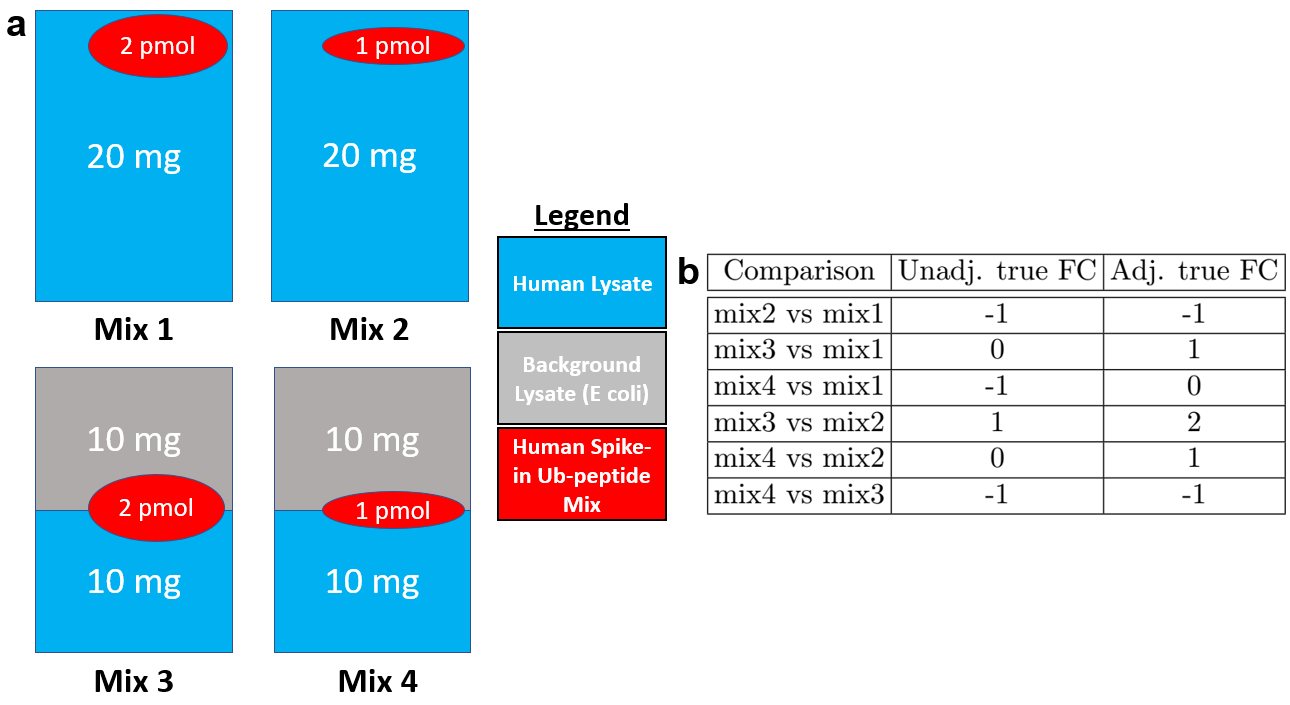
\includegraphics[scale=.5]{images/benchmark_fig.png}
\caption{{\bf Dataset 3: Spike-in benchmark - Ubiquitination - Label-free}. 
%
(a) Four mixtures (i.e., conditions) were created with varying amounts of human lysate, background {\it E. Coli} lysate, and human spike-in ub-peptide mixture. Unmodified peptides from human lysate were viewed as the global proteome. Background {\it E. coli} lysate were used to equalize total protein levels. 50 heavy-labeled KGG motif peptides from 20 human proteins were spiked into the mixed background of the lysates. Quantitative changes in protein and site abundance of these 20 human proteins were the target of the benchmark.
%
(b)  We distinguished the unadjusted changes (i.e. changes in the abundances of the modified peptides) and the protein-level adjusted changes of (i.e., changes in the abundances of the modified peptides relative to the changes in the abundances of the human lysate).   ``Unadj. true log$_2$FC'' are the log-ratios of the abundances of the spiked peptides between each condition. ``Adj. true log$_2$FC'' was calculated by determining the ratios of the abundances of the spiked peptides and human lysate between each condition and then adjusting the ratio of the spiked peptides by the human lysate, similarly to \eqref{null_hyp}.}
\label{fig:benchmark-design}
\end{figure}

\begin{figure}[ht]
\centering
\includegraphics[scale=.45]{images/fig3.png}
\caption{Schematic representation of one PTM site, in a special case of a label-free experiment with $I=2$ conditions and $J=2$ biological replicates per condition. After a log$_2$ transform, we are interested in estimating the difference between the population-level PTM abundance between Condition 1 and Condition 2 (i.e, $\mu^*_1-\mu^*_2$), relative to the population-level difference of the overall protein abundance (i.e., $\mu_1-\mu_2$).  These quantities are characterized by the observed spectral Features (boxes), i.e. peptides of different charge states. The peptides can be fully cleaved (solid lines), or partially cleaved (dashed lines). The log$_2$-intensities of the modified peptides in Condition $i$, Run $j$, and Feature $k$ are denoted by $y_{ijk}^{\ast}$. The log$_2$-intensities of Feature $k$ corresponding to the unmodified peptide in Condition $i$ and Run $j$ are denoted by $y_{ijk}$. }
\label{fig:data-structure}
\end{figure}


\begin{figure}[ht]
\centering
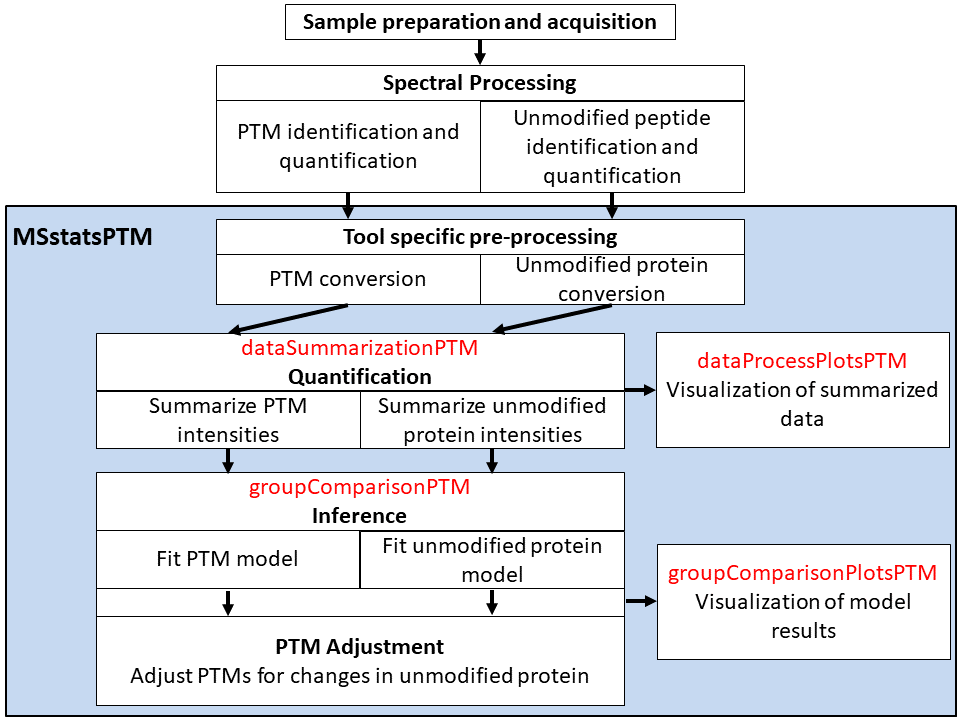
\includegraphics[scale=.5]{images/MSstatsPTM_design.png}
\caption{The $MSstatsPTM$ workflow. The names of the R functions used for each step are highlighted in purple and the output notations are highlighted in red. The workflow begins with the acquisition of the enriched and global proteome lysates. The package is applicable to label-free data acquisitions such as DDA, DIA, SRM and label-based data acquisitions such as TMT. It takes as input lists of identified and quantified spectral features for the PTM and unmodified protein, produced by spectral processing tools such as MaxQuant, Progenesis, or Spectronaut.  Conversion, summarization and statistical modeling are performed separately for the PTM and for the unmodified proteins. At the end, the model-based summaries are combined to adjust the changes in the PTM abundance for changes in unmodified protein abundance. Data visualizations can optionally be created after steps 4 and 5 of the workflow.}
\label{fig:msstatsptm_design}
\end{figure}

\begin{figure}[ht]
\centering
\begin{subfigure}[c]{0.7\linewidth}
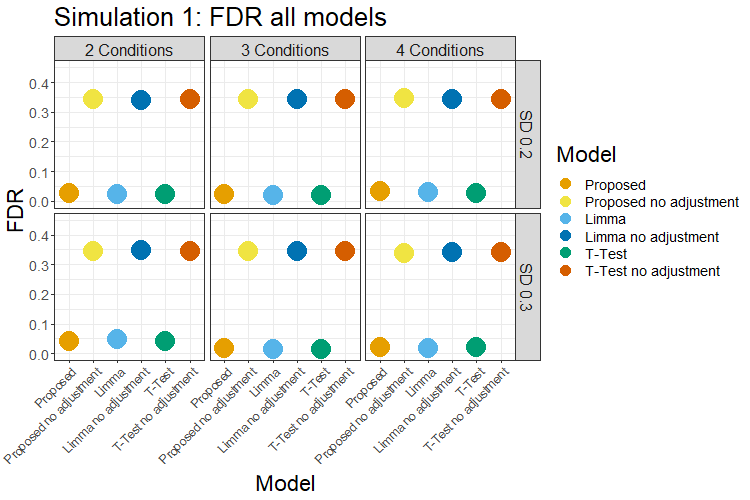
\includegraphics[width=1\textwidth]{images/sim1_FDR_all_models.png}
\caption{}
\label{fig:sim1_fdr}
\end{subfigure}
\begin{subfigure}[c]{0.825\linewidth}
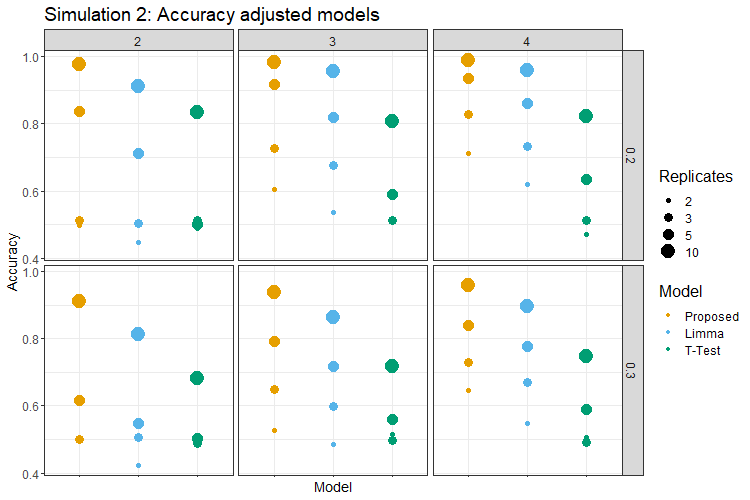
\includegraphics[width=1\textwidth]{images/sim3_Accuracy.png}
\caption{}
\label{fig:sim2_acc}
\end{subfigure}
\caption{Dataset 1 \& 2: Computer simulation. a) In a clean simulation, all the considered methods in the first computer simulation correctly calibrated FDR when adjusting for changes in protein abundance. In comparison, the methods without accounting for the protein-level changes resulted in off-target, high false positive rates. b) In a noisy simulation, including limited feature observations and missing values, the advantage of the proposed approach was apparent. Looking at accuracy, the proposed method outperformed ANOVA and Limma in nearly every model.
}
\label{fig:computer_sim}
\end{figure}


\begin{figure}[ht]
\centering
\begin{subfigure}[c]{0.825\linewidth}
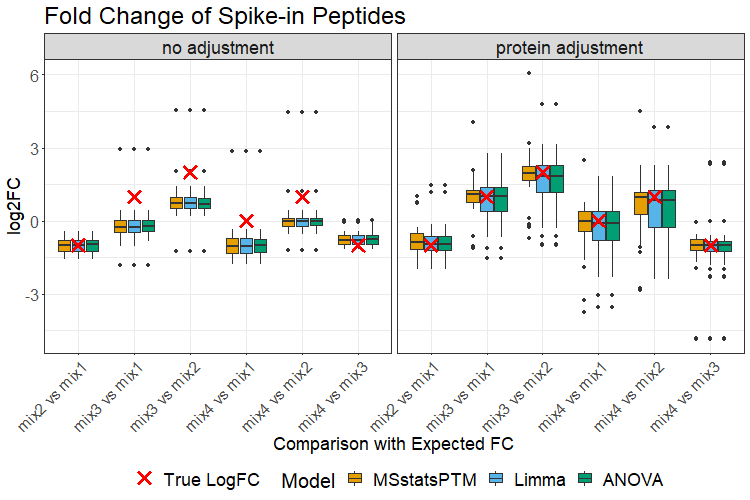
\includegraphics[width=1\textwidth]{images/spike_in_fc.png}
\caption{}
\label{fig:spikein_boxplot}
\end{subfigure}
\begin{subfigure}[c]{0.825\linewidth}
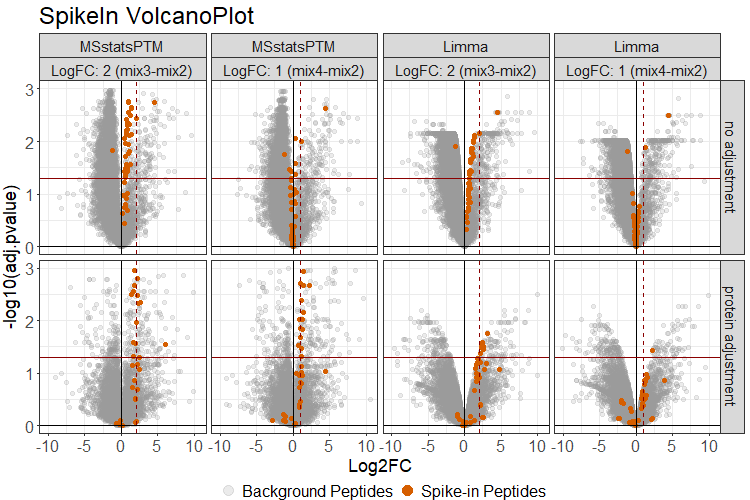
\includegraphics[width=1\textwidth]{images/spike_in_volcano.png}
\caption{}
\label{fig:spikein_prop_volcano}
\end{subfigure}
\caption{Dataset 3: Spike-in benchmark - Ubiquitination - Label-free. a) Before adjustment the fold change of the spike-in peptides' were systematically different from the expected fold change in all models. After adjustment, this systemic difference was removed, however the inner quartile range of the Limma and ANOVA models was wider than the proposed method. b) Before adjustment the spike-in peptides (colored red) did not follow the expected log fold change; after adjustment, the spike-in peptides were more in line with expectation. Using Limma, the spike-in peptides followed the expected log fold change after adjustment, however the majority of spike-in peptides did not have a significant adjusted p-value.}
\label{fig:spikein_volcano}
\end{figure}

\begin{figure}[ht]
\centering
\begin{subfigure}[c]{0.55\linewidth}
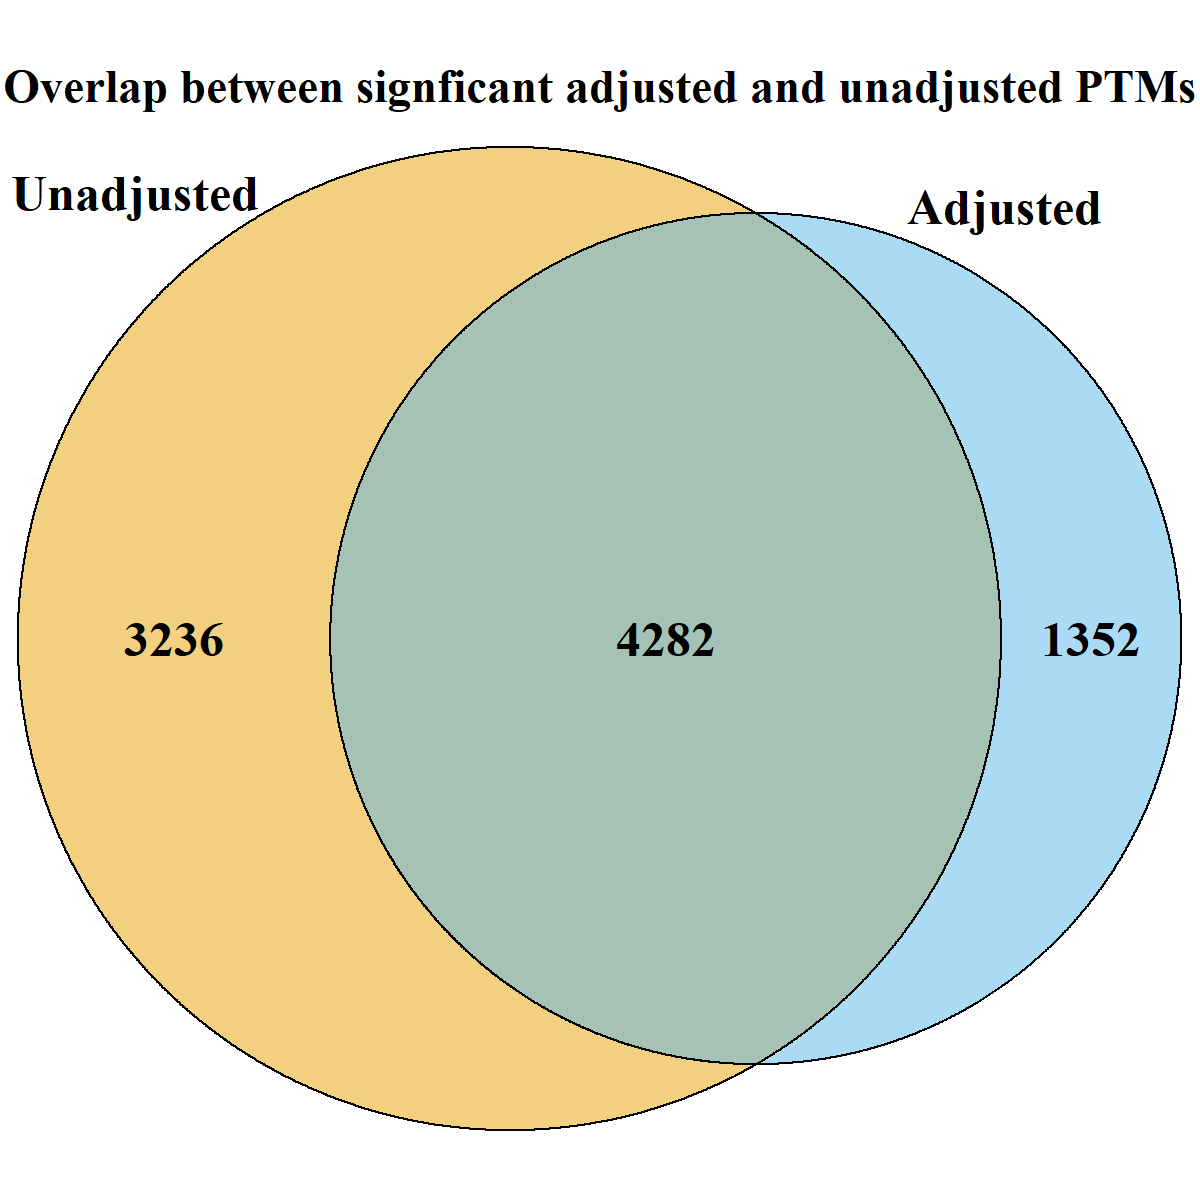
\includegraphics[width=1\textwidth]{images/ipah_venn_diagramm.png}
\caption{}
\label{fig:data4_venn_diagram}
\end{subfigure}
\begin{subfigure}[c]{0.55\linewidth}
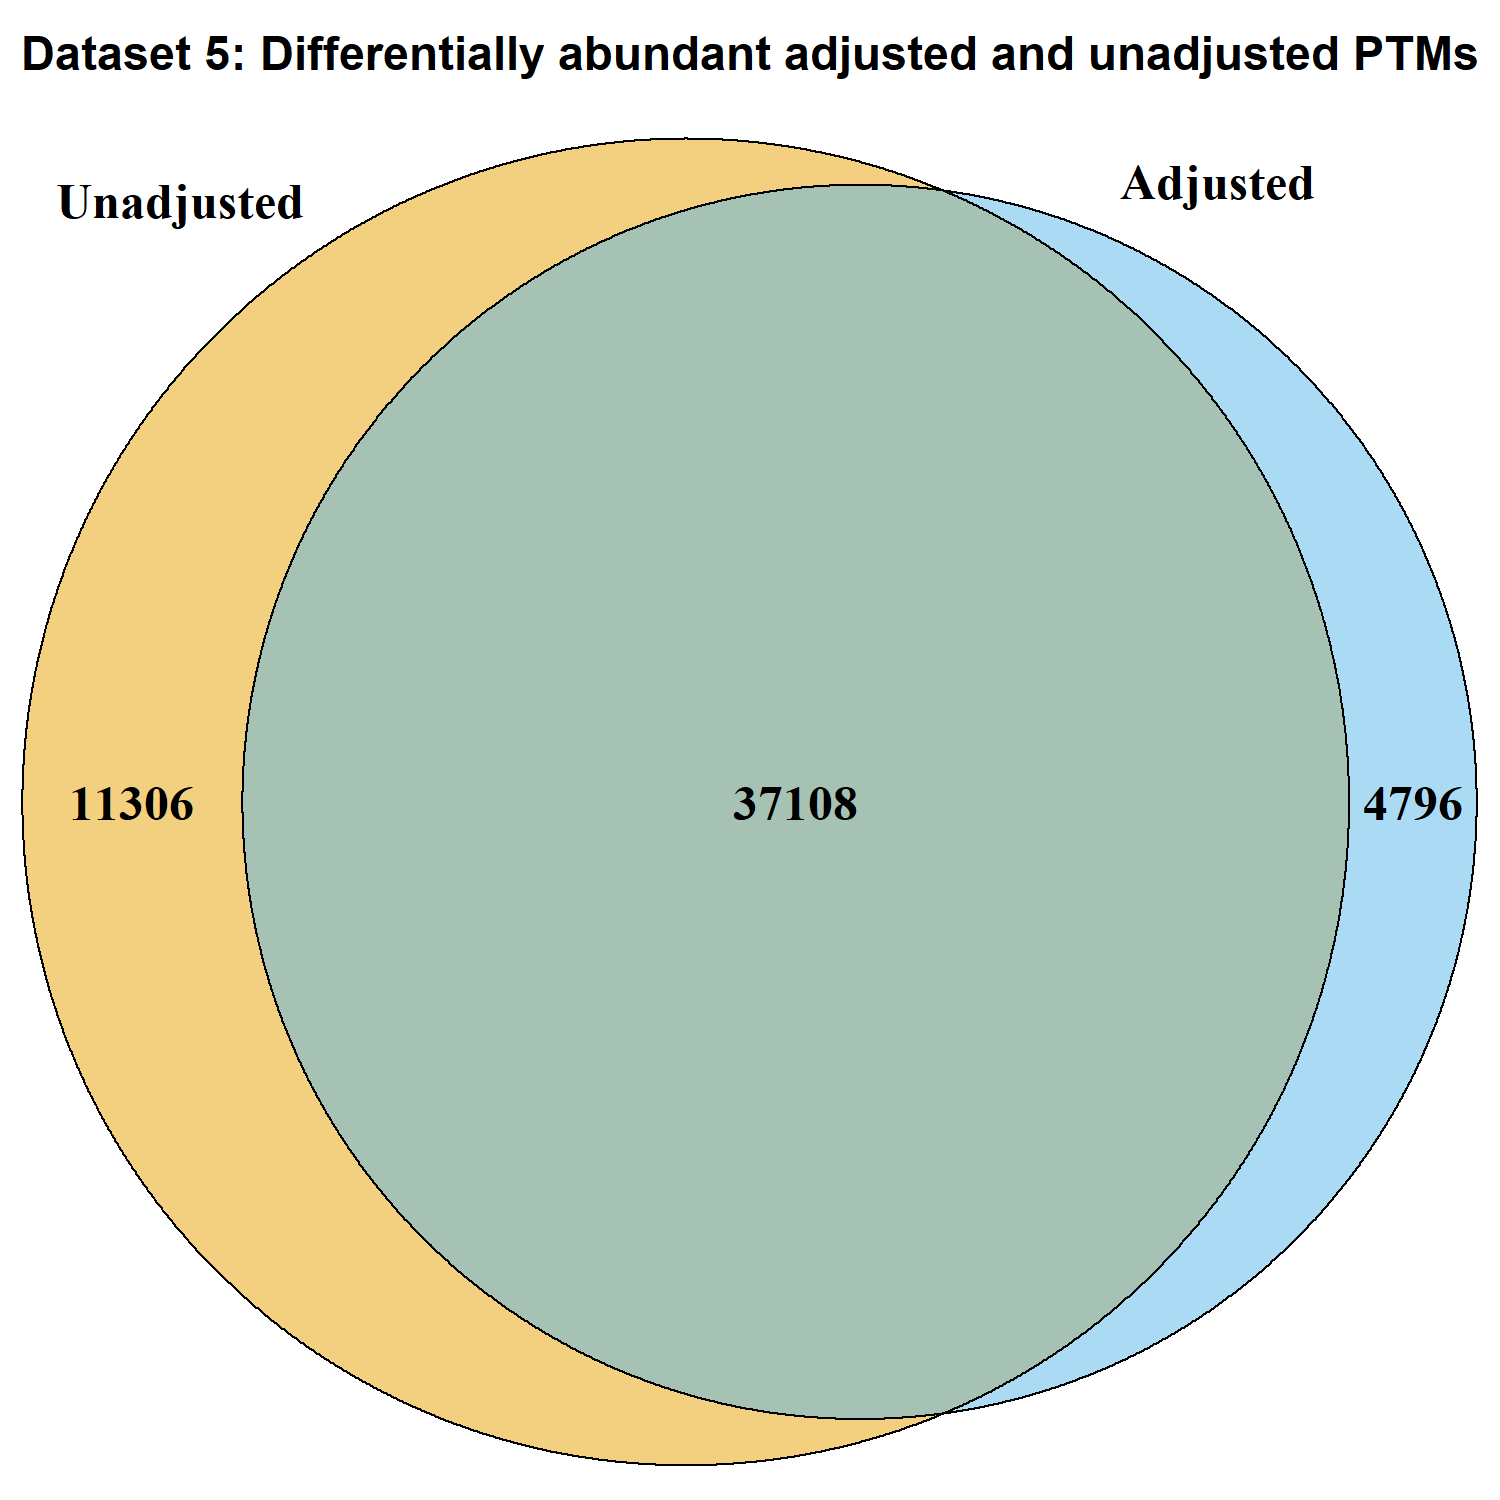
\includegraphics[width=1\textwidth]{images/shig_venn_diagramm.png}
\caption{}
\label{fig:data5_venn_diagram}
\end{subfigure}
\caption{
a) Dataset 4: Human - Ubiquitination - 1mix-TMT. The overlap of differential modified peptides for the PTM model with and without global protein level adjustment across all comparisons.  3,236 modified peptides became insignificant, 1,352 became significant, while 4,282 were significant in both models. b) Dataset 5: Mouse - Phosphorylation - 2mix-TMT. The overlap of differentially modified peptides between the PTM model with and without global protein level adjustment across all comparisons. 19,286 peptides became insignificant, 4,947 became significant, and 41,552 were significant in both models. }
\label{fig:venn_diagrams}
\end{figure}

\begin{figure}[h!]
\centering
\begin{subfigure}{\textwidth}
 \centering
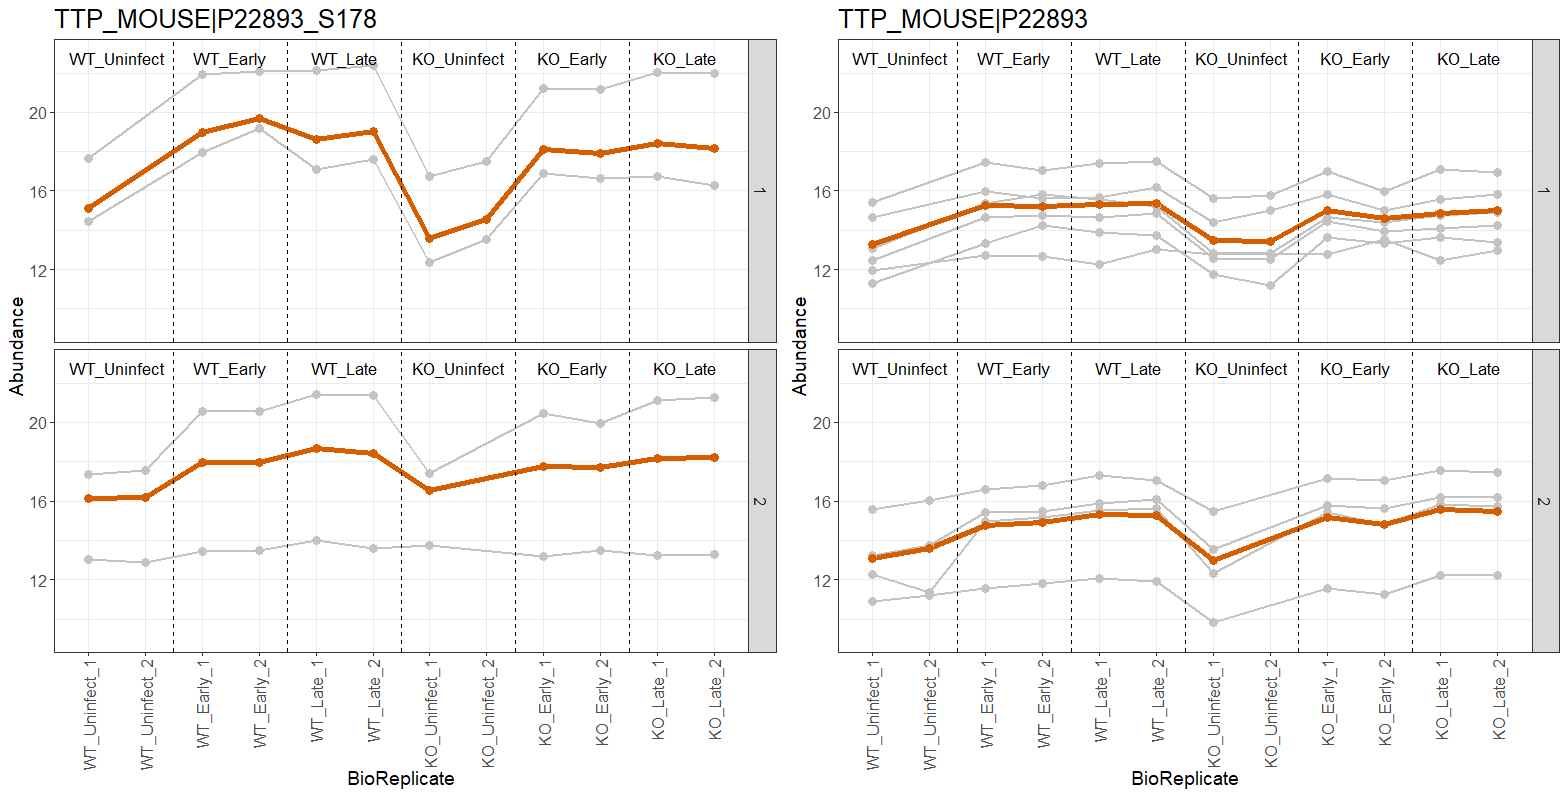
\includegraphics[width=1.0\textwidth]{images/No_Difference_Shigella_Profile_Plot}
\caption{}
\label{fig:data4_profile_plot}
 \end{subfigure}
 \begin{subfigure}{\textwidth}
 \centering
	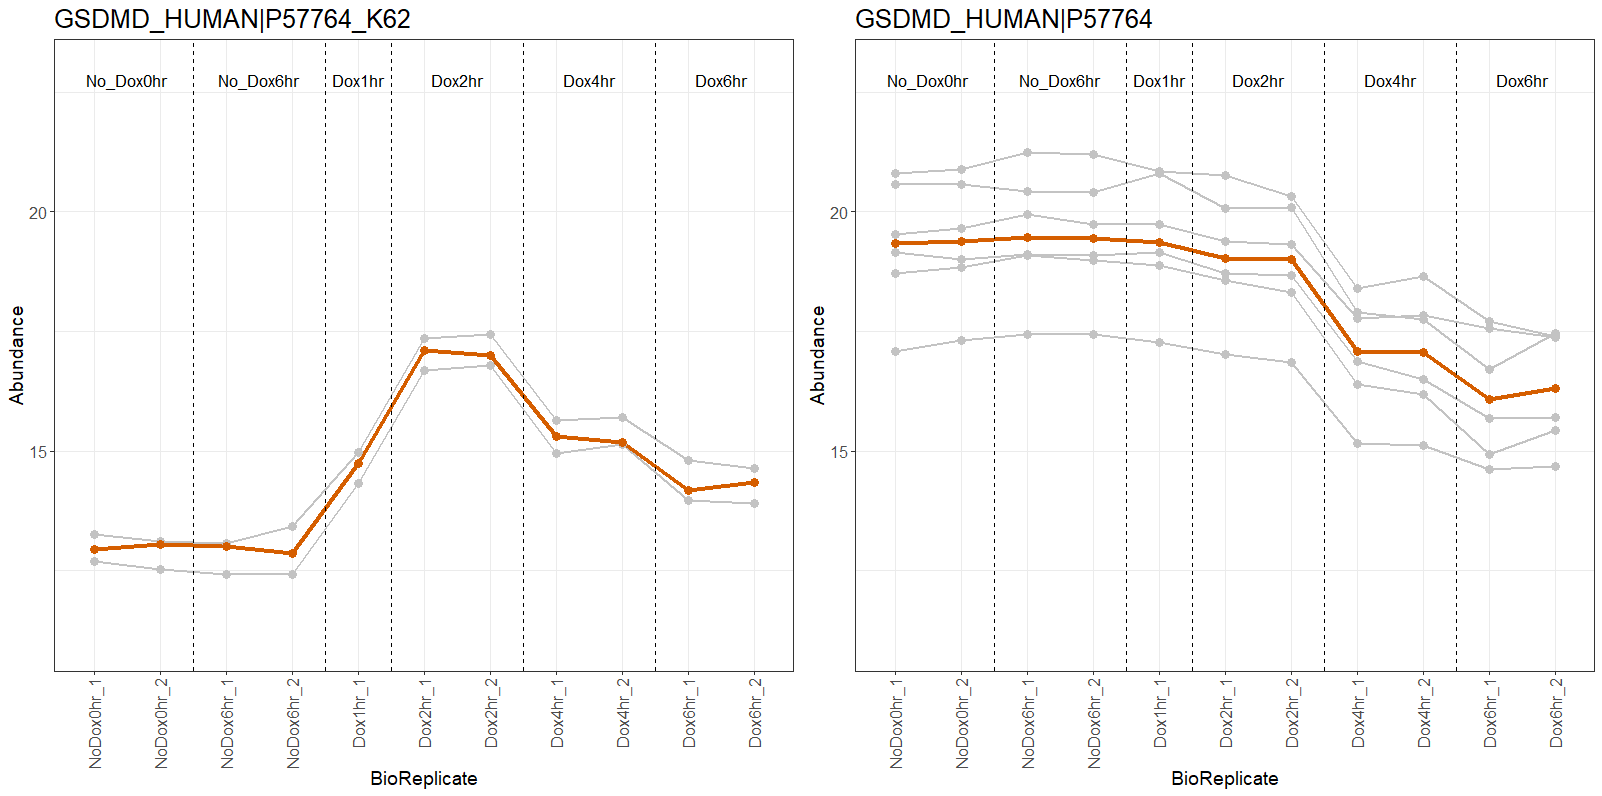
\includegraphics[width=1.0\textwidth]{images/IpaH_prof_plot.png}
	\caption{}
	\label{fig:data5_profile_plot}
	 \end{subfigure}
\caption{a) Dataset 5: Mouse - Phosphorylation - 2mix-TMT. Comparing the global profiling of protein $TTP$ with the modification at site $S178$. The modification and unmodified protein abundance followed the same trend across conditions. Specifically, there was a positive adjustment in abundance when comparing WT\_Uninfect to WT\_Late in both the modification and global profiling run. b) Dataset 4: Human - Ubiquitination - 1mix-TMT. Comparing the global profiling of protein $GSDMD$ with the ubiquitination of the protein at site $K62$. Here the modification and global protein follow different trends. There appeared to be no change in abundance between Dox1hr and Dox4hr in the modified plot, however there was a large negative change when looking at the unmodified plot. This indicated the modification was confounded with changes in the unmodified protein.}
\label{fig:profile_plots}
\end{figure}

\begin{figure}[h!]
\centering
 \begin{subfigure}{\textwidth}
 \centering
	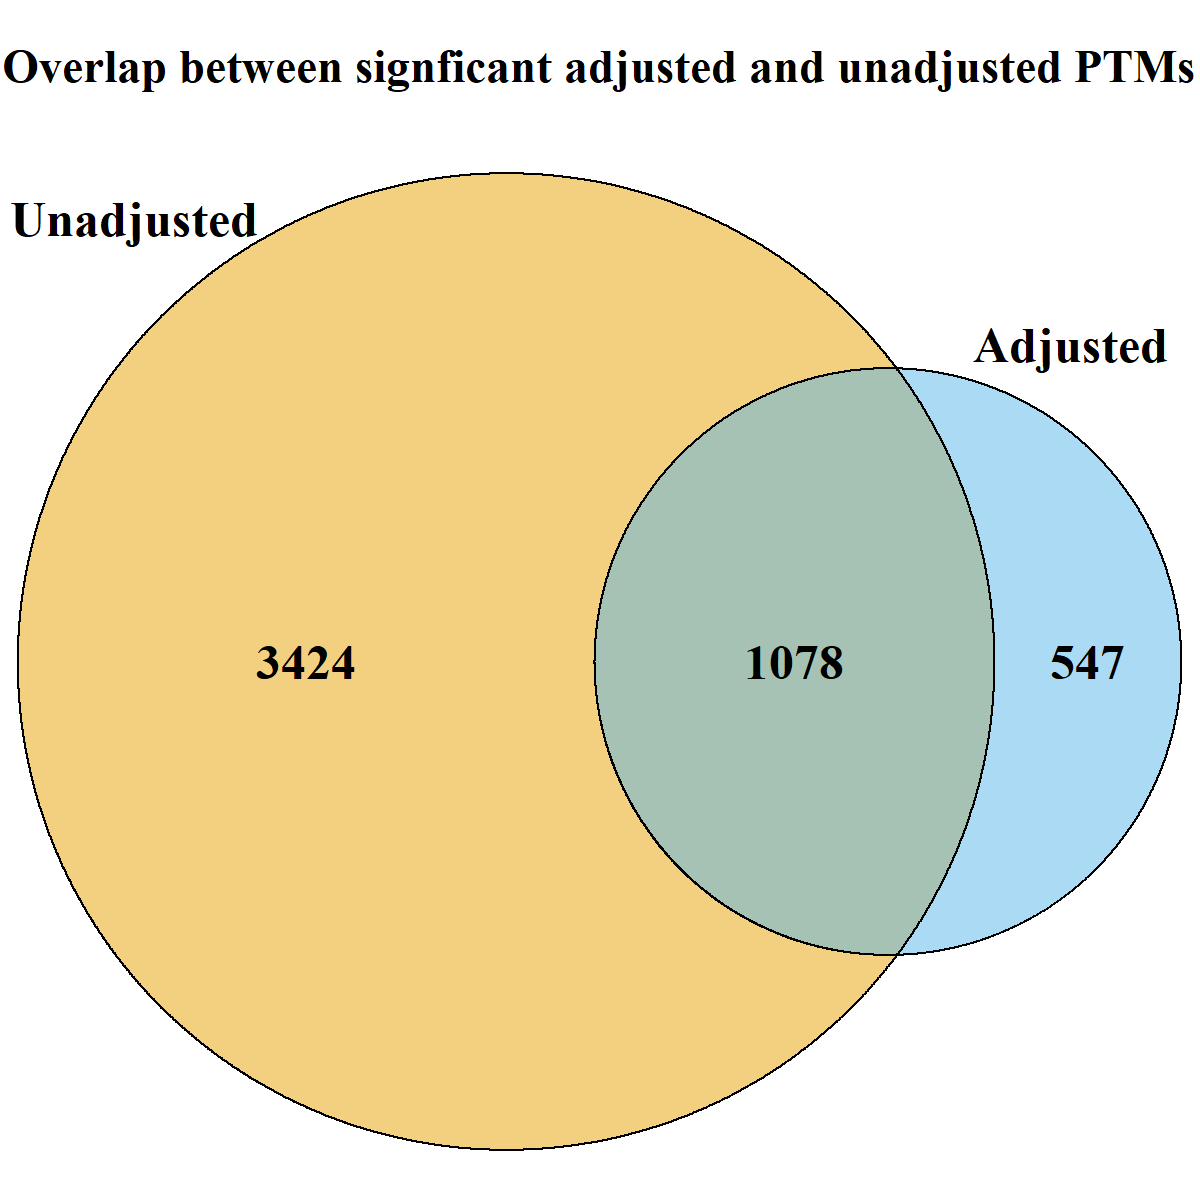
\includegraphics[height=.55\textwidth]{images/usp30_venn_diagramm}
	\caption{}
	\label{fig:data6_vd1}
 \end{subfigure}
 \begin{subfigure}{\textwidth}
 \centering
	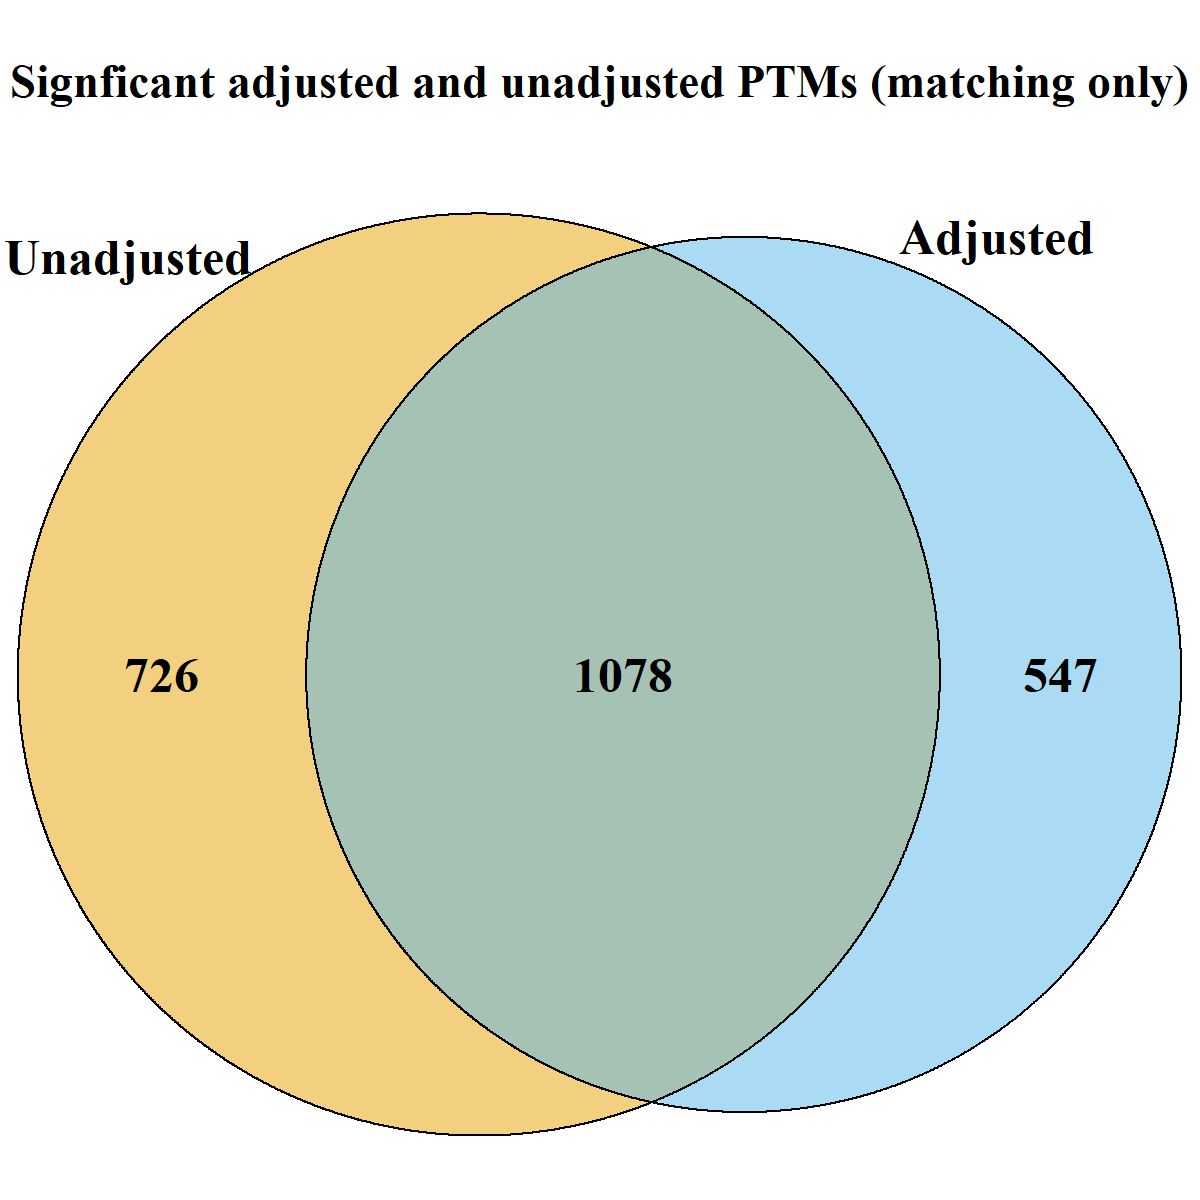
\includegraphics[height=.55\textwidth]{images/usp30_venn_diagramm_matching_only}
	\caption{}
	\label{fig:data6_vd2}
 \end{subfigure}
 \caption{Dataset 6: Human - Ubiquitination - Label-free no global profiling run. a) The overlap of differential modified peptides for the PTM model with and without global protein level adjustment across all comparisons. More PTMs became insignificant than became significant after adjustment. In total, 2709 modified peptides became insignificant, while only 547 became significant. b) Here we made the same comparison but only looked at modified peptides where adjustment could be performed, ie they had a matching unmodified protein. In this case there were significantly less peptides that became insignificant after adjustment. 726 modified peptides became insignificant, 547 became significant, and 1,078 were significant in both models.}
\label{fig:data6_plots}
\end{figure}

%\begin{figure}[h!]
%\centering
% \begin{subfigure}{\textwidth}
% \centering
%	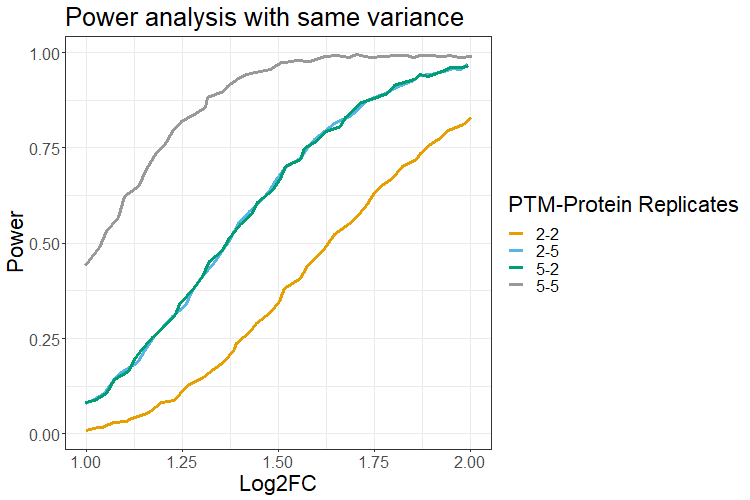
\includegraphics[width=.75\textwidth]{images/same_var_power}
%	\caption{}
% \end{subfigure}\vspace{5mm}
% \begin{subfigure}{\textwidth}
% \centering
%	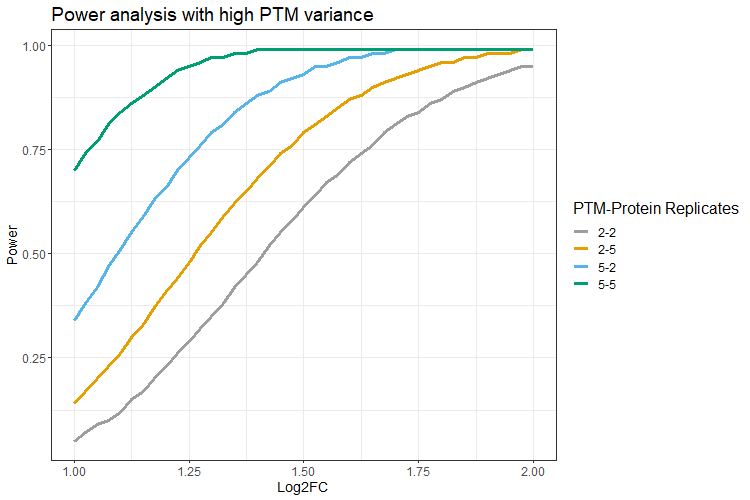
\includegraphics[width=.75\textwidth]{images/high_ptm_var_power}
%	\caption{}
% \end{subfigure}
% \caption{Power analysis of experiments with differing variances. a) The power of an experiment targeting PTMs with the same variance, .15, for the modified and unmodified peptides. Predictably when the replicates are high for both modified and unmodified peptides the power is much higher. Conversely at low replicates for each the power is much lower. The interesting part of this chart is when the replicates are different between runs. With equal variance, it does not matter if the PTM replicates or protein replicates are higher. b) In this chart the variance for the PTM is higher than the unmodified protein. The PTM variance is .2, while the unmodified protein variance is .1. With equal replicates the results are the same as above, more replicates equals more power. When the replicates are not the same we can clearly see that having more replicates for the PTM leads to higher power.}
%\label{fig:power_sd_combo}
%\end{figure}


\end{document}
